\subsection{Z+X Background}

We define the following naming conventions in this appendix:

\begin{itemize}
    \item \zx: the sum of the Drell-Yan, \wz~and \zz~processes.
    \item \zv: the diboson processes, \wz~and \zz.
    \item On-resonance: the dilepton invariant mass is within the \z~mass window
    \item Off-resonance: the dilepton invariant mass is outside of the \z~mass window.
The exact mass region used for the signal selection depends on the Higgs boson mass.
    \item MET: the minimum of projected trackerMET and PFMet, as used in the usual analysis selection.
\end{itemize}

We perform a Higgs boson search in the di-lepton + MET final state using 1.1~fb$^{-1}$ of data.
If both leptons are required to have the same flavor ($e^{+}e^{-}$ or $\mu^{+}\mu^{-}$)
then a large background may be introduced from processes with the final state \zx.
These backgrounds are reduced by vetoing events where the dilepton invariant mass
is consistent with the \z~boson.

The remaining Drell-Yan contribution to the off-resonance region
arises when fake MET is generated by the mis-meausrement of 
one or both of the leptons, recoiling hadronic jets if present, or instrumental noise.
Because we do not necessarily expect the fake MET distribution to be well reproduced by the simulation
we need to define a data driven technique to estimate the Drell-Yan background.
The level of agreement between the simulation and data is illustrated for the on-resonance
control region at \ww~preselection level in Figure \ref{fig:sample_composition}.

Additional contributions to the off-resonance region arise from the diboson processes, \wz~and \zz.
Because the decay of the second boson can produce real MET, 
the contribution of these processes is large.
This contributes more than a half of the \zx~background at the \ww~preselection level as illustrated in Figure \ref{fig:sample_composition}.
However, real MET should be well reproduced by the simulation, thus we can estimate
the \zv~contribution from simulation with appropriate systematic uncertainties 
on the production cross sections.
The expected contributions from \zv~and Drell-Yan are compared with the same flavor
yields in data for the zero and one-jet bins in Tables \ref{tab:results_nin_0j} and \ref{tab:results_nin_1j} respectively.

\begin{figure}[h!]
\begin{center}$
\begin{array}{cc}
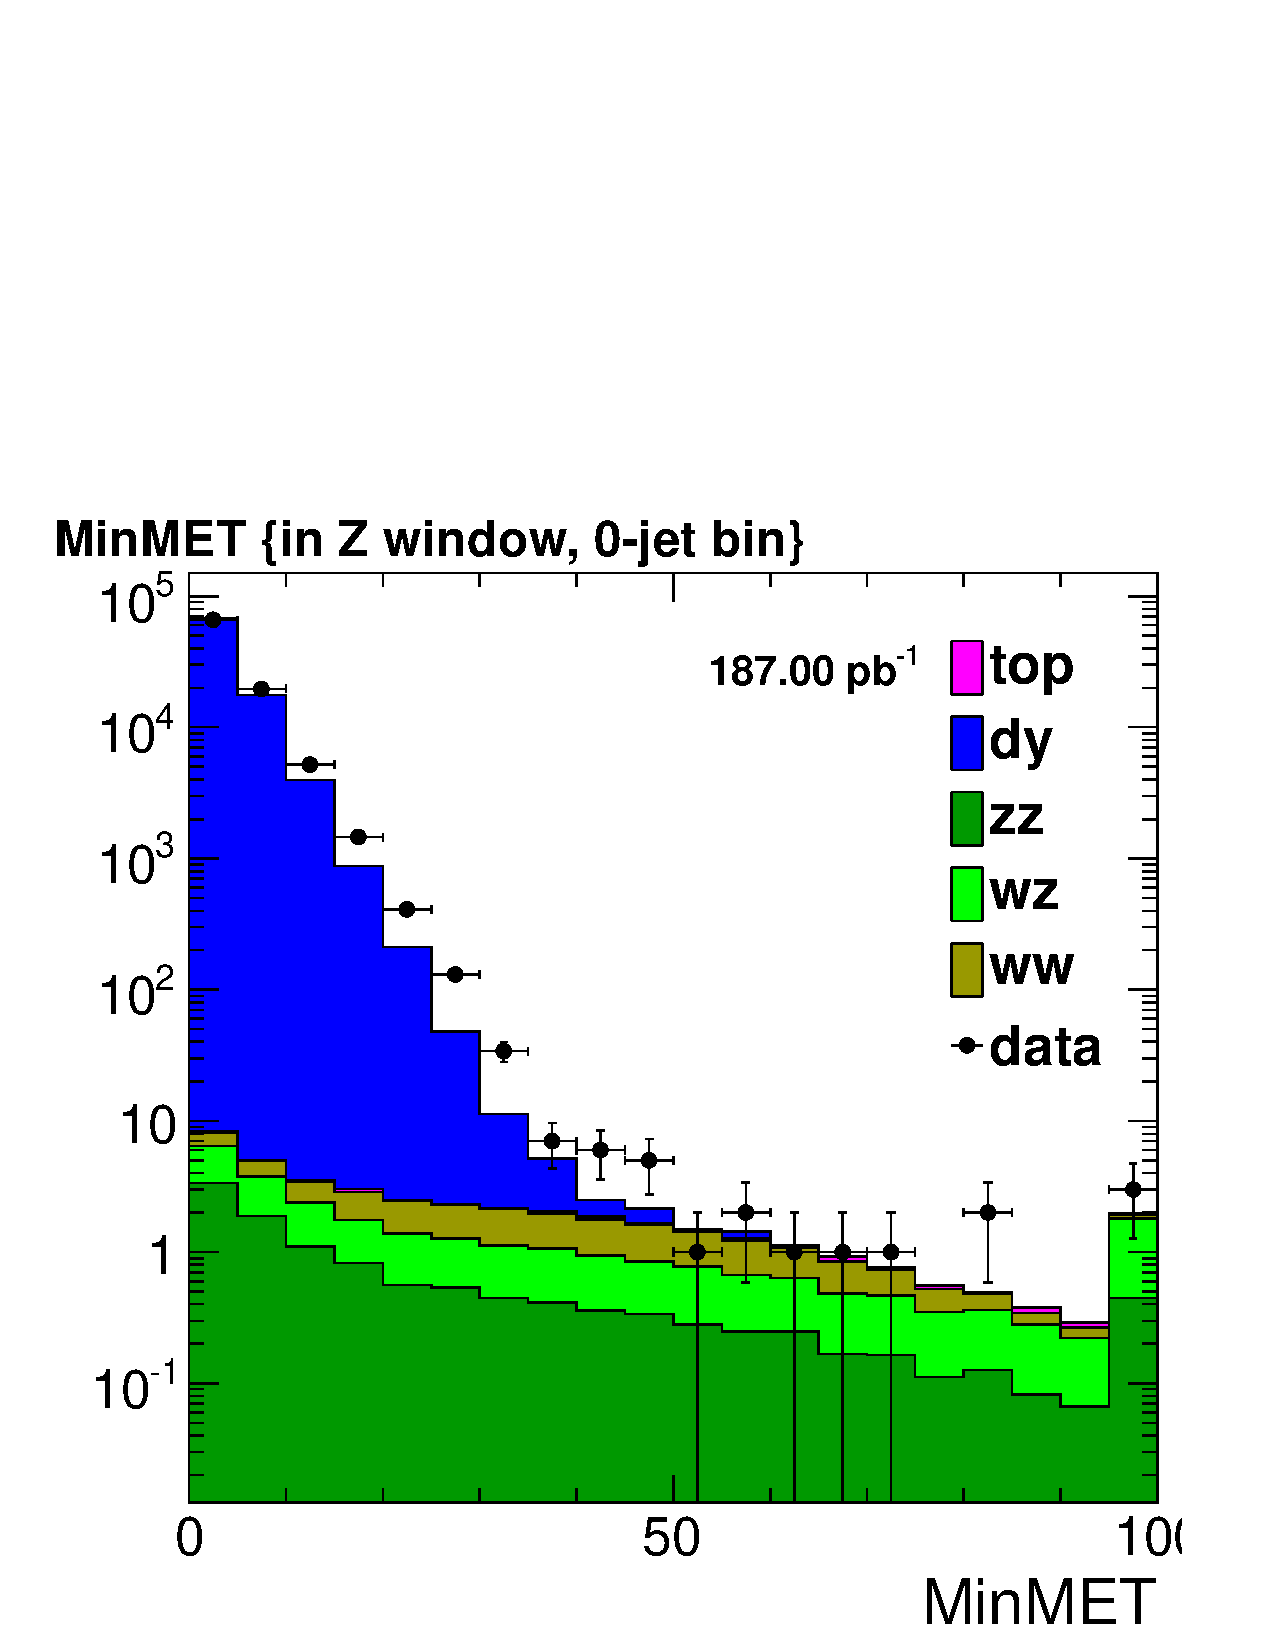
\includegraphics[width=.47\textwidth]{figures/met_agreement.pdf} &
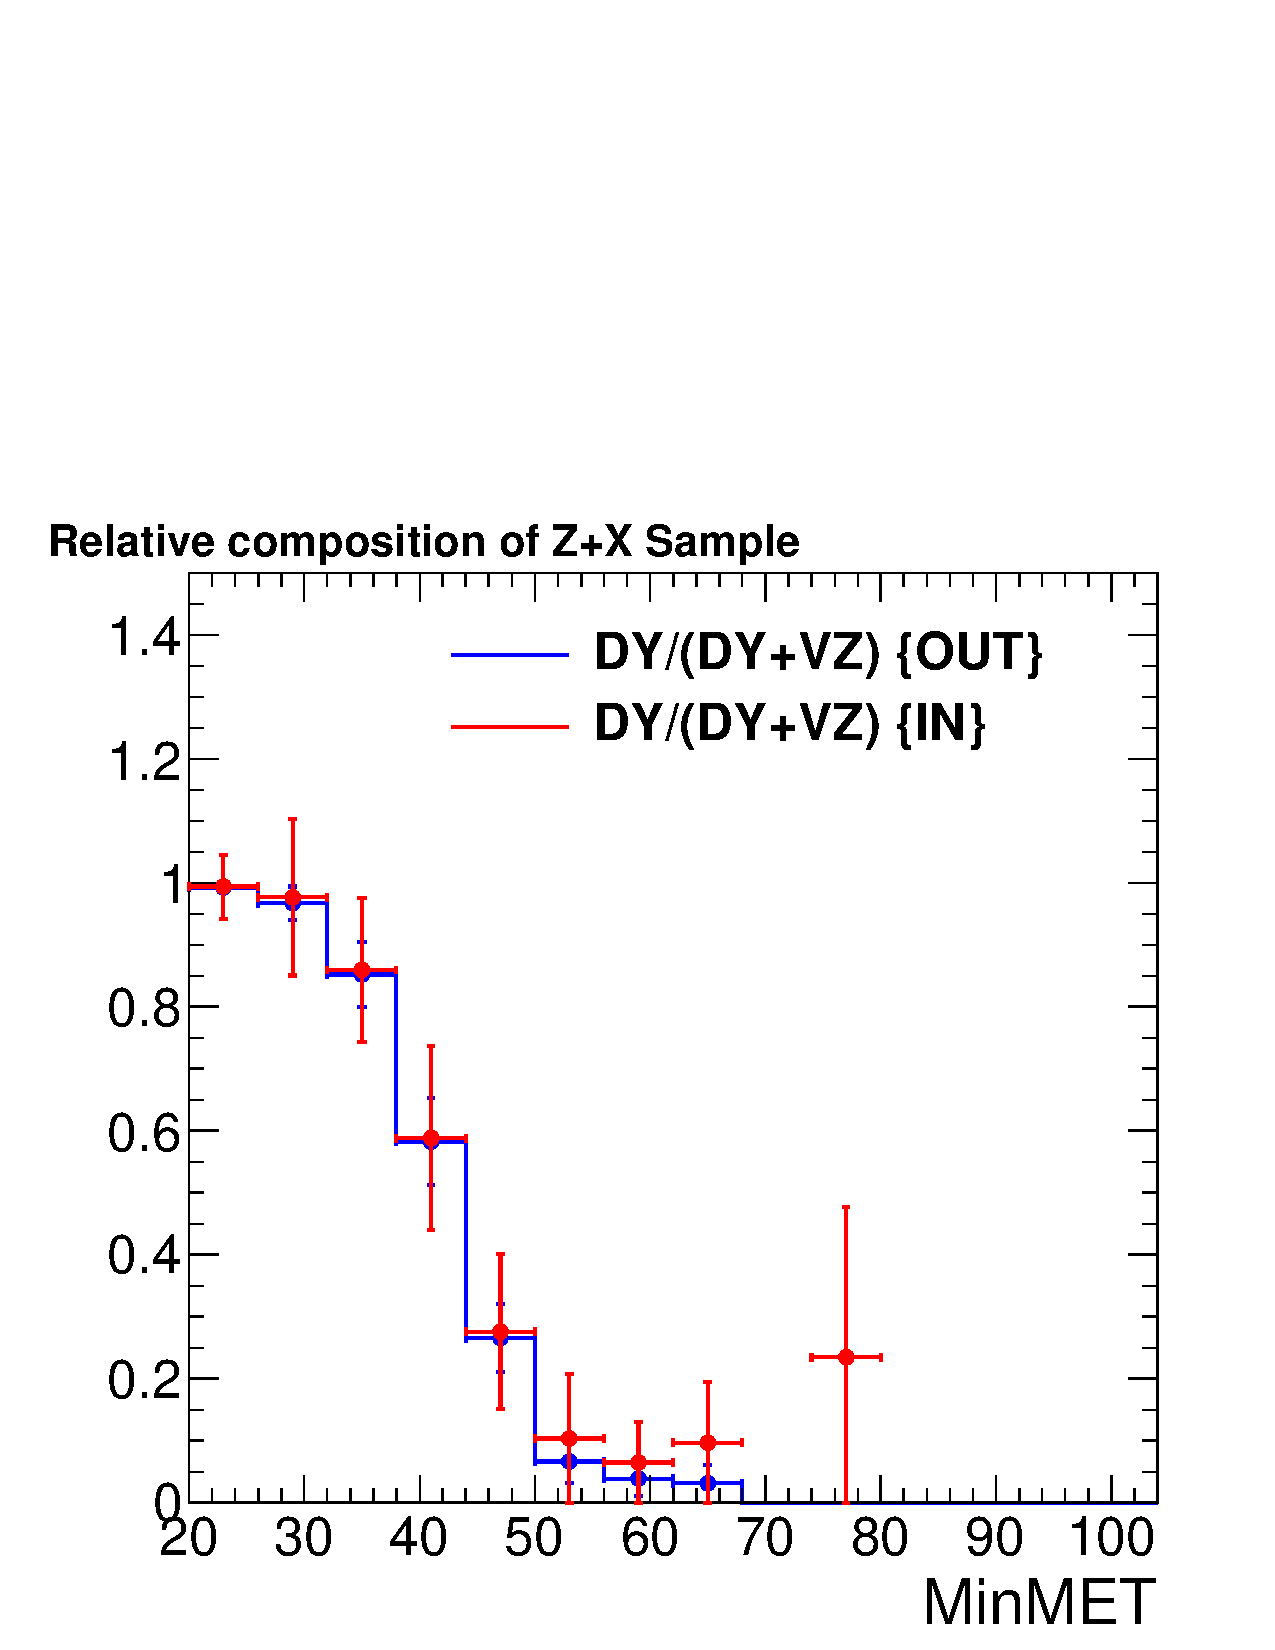
\includegraphics[width=.47\textwidth]{figures/relative_composition.pdf}
\end{array}$
\end{center}
\caption{The expected on-resonance control region in the 187 pb$^{-1}$ data sample compared to simulation as a function of MET (left). 
The relative \zx~sample composition in simulation as a function of MET (right).}
\label{fig:sample_composition}
\end{figure}

%%%%%%
\vspace{10pt}
\begin{table}[!ht]
\begin{center}
\begin{tabular}{c|c|c c}
\hline
Analysis  & $N^{data}_{in}$(\zx) & $N^{mc}_{in}$(\zv) & $N^{mc}_{in}(\mathrm{DY})$ \\ 
\hline
 \ww\, & 70.61 $\pm$ 12.44 & 44.97 $\pm$ 0.51 & 7.92 $\pm$ 0.89\\
 mH = 120 GeV  & 16.62 $\pm$ 6.31 & 5.19 $\pm$ 0.18 & 3.24 $\pm$ 0.58\\
 mH = 130 GeV  & 1.76 $\pm$ 4.06 & 2.09 $\pm$ 0.11 & 1.25 $\pm$ 0.35\\
 mH = 140 GeV  & 2.79 $\pm$ 3.93 & 2.09 $\pm$ 0.11 & 1.00 $\pm$ 0.31\\
 mH = 150 GeV  & 1.72 $\pm$ 4.31 & 2.18 $\pm$ 0.11 & 0.81 $\pm$ 0.27\\
 mH = 160 GeV  & 1.97 $\pm$ 2.02 & 0.79 $\pm$ 0.07 & 0.25 $\pm$ 0.15\\
 mH = 170 GeV  & 2.93 $\pm$ 2.67 & 0.89 $\pm$ 0.07 & 0.06 $\pm$ 0.06\\
 mH = 180 GeV  & 1.86 $\pm$ 3.21 & 1.45 $\pm$ 0.09 & 0.13 $\pm$ 0.09\\
 mH = 190 GeV  & 8.79 $\pm$ 4.63 & 4.10 $\pm$ 0.15 & 0.25 $\pm$ 0.13\\
 mH = 200 GeV  & 11.72 $\pm$ 5.34 & 7.47 $\pm$ 0.21 & 0.56 $\pm$ 0.22\\
 mH = 250 GeV  & 18.65 $\pm$ 6.30 & 16.56 $\pm$ 0.31 & 0.62 $\pm$ 0.23\\
 mH = 300 GeV  & 12.90 $\pm$ 4.38 & 12.33 $\pm$ 0.26 & 0.44 $\pm$ 0.21\\
% mH = 350 GeV  & 8.97 $\pm$ 3.33 & 8.96 $\pm$ 0.22 & 0.31 $\pm$ 0.19\\
% mH = 400 GeV  & 4.97 $\pm$ 2.66 & 5.92 $\pm$ 0.18 & 0.31 $\pm$ 0.19\\
% mH = 450 GeV  & 1.97 $\pm$ 2.02 & 2.58 $\pm$ 0.11 & 0.19 $\pm$ 0.14\\
% mH = 500 GeV  & 2.00 $\pm$ 1.41 & 1.82 $\pm$ 0.10 & 0.19 $\pm$ 0.14\\
% mH = 550 GeV  & 2.00 $\pm$ 1.41 & 1.36 $\pm$ 0.08 & 0.12 $\pm$ 0.12\\
% mH = 600 GeV  & 3.00 $\pm$ 1.73 & 1.02 $\pm$ 0.07 & 0.12 $\pm$ 0.12\\
\hline
\end{tabular}
\caption{The number of same flavor events inside the Z mass window measured 
in data after the opposite flavor subtraction in the 0-Jet bin. 
We compare this measurement with the MC expectation from Drell-Yan and 
the resonant component of \zv~processes. 
The comparisons are performed after both \ww~and higgs selections with 
various higgs mass hypotheses. 
}
\label{tab:results_nin_0j}
\end{center}
\end{table}
%%%%%%

%%%%%%
\vspace{10pt}
\begin{table}[!ht]
\begin{center}
\begin{tabular}{c|c|c c}
\hline
Analysis  & $N^{data}_{in}$(\zx) & $N^{mc}_{in}$(\zv) & $N^{mc}_{in}(\mathrm{DY})$ \\ 
\hline
 \ww\, & 67.26 $\pm$ 10.56 & 16.52 $\pm$ 0.33 & 22.26 $\pm$ 1.48\\
 mH = 120 GeV  & 16.00 $\pm$ 4.00 & 1.79 $\pm$ 0.11 & 9.91 $\pm$ 0.99\\
 mH = 130 GeV  & 4.96 $\pm$ 2.66 & 0.94 $\pm$ 0.08 & 5.86 $\pm$ 0.79\\
 mH = 140 GeV  & 4.96 $\pm$ 2.66 & 1.15 $\pm$ 0.09 & 6.73 $\pm$ 0.83\\
 mH = 150 GeV  & 13.93 $\pm$ 4.26 & 1.48 $\pm$ 0.10 & 7.23 $\pm$ 0.84\\
 mH = 160 GeV  & 3.89 $\pm$ 3.20 & 0.63 $\pm$ 0.07 & 2.62 $\pm$ 0.51\\
 mH = 170 GeV  & 4.89 $\pm$ 3.35 & 0.66 $\pm$ 0.07 & 2.12 $\pm$ 0.46\\
 mH = 180 GeV  & 3.86 $\pm$ 3.51 & 0.98 $\pm$ 0.08 & 2.12 $\pm$ 0.45\\
 mH = 190 GeV  & 13.86 $\pm$ 4.72 & 2.49 $\pm$ 0.13 & 5.30 $\pm$ 0.72\\
 mH = 200 GeV  & 20.82 $\pm$ 5.60 & 3.65 $\pm$ 0.16 & 6.55 $\pm$ 0.80\\
 mH = 250 GeV  & 29.82 $\pm$ 6.35 & 6.40 $\pm$ 0.21 & 6.61 $\pm$ 0.79\\
 mH = 300 GeV  & 22.96 $\pm$ 5.01 & 5.31 $\pm$ 0.19 & 5.36 $\pm$ 0.72\\
% mH = 350 GeV  & 20.00 $\pm$ 4.47 & 3.99 $\pm$ 0.16 & 3.74 $\pm$ 0.60\\
% mH = 400 GeV  & 14.00 $\pm$ 3.74 & 2.91 $\pm$ 0.14 & 2.68 $\pm$ 0.51\\
% mH = 450 GeV  & 4.00 $\pm$ 2.00 & 1.36 $\pm$ 0.09 & 1.25 $\pm$ 0.34\\
% mH = 500 GeV  & 2.00 $\pm$ 1.41 & 1.01 $\pm$ 0.08 & 0.69 $\pm$ 0.26\\
% mH = 550 GeV  & 1.00 $\pm$ 1.00 & 0.79 $\pm$ 0.07 & 0.56 $\pm$ 0.22\\
% mH = 600 GeV  & 1.00 $\pm$ 1.00 & 0.65 $\pm$ 0.06 & 0.44 $\pm$ 0.21\\
\hline
\end{tabular}
\caption{The number of same flavor events inside the Z mass window measured 
in data after the opposite flavor subtraction in the 1-Jet bin. 
We compare this measurement with the MC expectation from Drell-Yan and 
the resonant component of \zv~processes. 
The comparisons are performed after both \ww~and higgs selections with 
various higgs mass hypotheses. 
}
\label{tab:results_nin_1j}
\end{center}
\end{table}
%%%%%%

We now describe the data driven estimation of the Drell-Yan background.

%
%
%
\subsubsection{Review of Methods to Estimate the Drell-Yan Background}

All methods of the Drell-Yan background estimation exploit the fact
the Drell-Yan events decay only to the same-flavor final states. All
other Standard Model processes contribute equally to the same-flavor
and the opposite-flavor final states. In principle the Drell-Yan
background can be measured by simply counting events in the
same-flavor final states and subtracting events in the opposite-flavor
final states. In practice it only works well if the same-flavor event
count is much larger than the opposite-flavor one. Otherwise we have a
case of measuring a small number by subtracting two large numbers,
which leads to a result with a very large statistical uncertainty. If we
look at the Z-peak region we keep most of Drell-Yan events in the
same-flavor final state, while dramatically reducing the event yield
in the opposite-flavor final states.

Because we veto the same flavor on-resonance events in the analysis to reduce the \zx~background
we can use these events as a control region to estimate the residual background.
This has been done successfully in other experiments such as CDF, and in previous CMS analyses  following the method described
in AN2009/023, usually referred to as the ``\routin'' method.

In this method, the residual Drell-Yan background is estimated from the number of Drell-Yan events 
in the on-resonance region in data.
This is determined
by subtracting the top and \ww~contributions using the $e\mu$ final state as described in AN2009/023.
We subtract the \zv~contribution using simulation.
The Drell-Yan simulation is then used to estimate the off-resonance contribution by normalising to
the on-resonance measurement. 
%The \zv~contribution to the off-resonance region will also be taken from simulation and is not
%discussed further here.
%In what follows we only consider the data driven estimation of the Drell-Yan background.

For convenience in defining the uncertainty on the simulation of the
Drell-Yan line shape, we define \routin~as the ratio of the off-resonance yield
to the on-resonance yield.
Thus the predicted Drell-Yan contribution in the off-resonance region $N(\mathrm{DY})^{data}_{out}$ is given by,

\begin{equation}
N(\mathrm{DY})^{data}_{out} = N^{data}_{in}(\mathrm{DY}) \cdot <\routin>.
\end{equation}

Where $N^{data}_{in}(\mathrm{DY}) = N^{data}_{in}(\zx) - N^{mc}_{in}(\zv)$. 
The \routin\, method relies on the assumption that the dependence of the \routin\, 
on the MET is well modelled by the simulation or relatively flat. 
The largest variations of the \routin\, with respect to the MET cut 
is then taken as the systematic uncertainty on the \routin. 

This measurement is performed for each of the Higgs boson mass dependent 
analysis selections, where $<\routin>$~~is the expected value of \routin
as derived from similation of each selection. 
Because the measurement is performed by counting events in data after the final
MET selection, the sensitivity to the description of the MET tail in data is minimised.
It is necessary to determine $<\routin>$~for each selection
because the differing kinematic requirements such as those on $\Delta\phi(l_1, l_2)$
will change the expected line shape, as well as the differing definitions of the
off-resonance region.
The assumption that the simulation can model the \zx~line shape has been 
validated using data.
This was done by comparing the \routin~in data after performing $e\mu$ subtraction, 
with the simulation expectations as a function of MET below the signal region MET cut.
Good agreement between data and simulation was found.

Because this analysis was initially performed with close to $200$~pb$^{-1}$, about
one fifth of the final data sample, the control region in data 
was statistically limited after the final selections.
Further, the Drell-Yan simulation sample used to predict \routin~was also 
initially statistically limited.  
For these reasons, we introduced a second method to estimate the \zx~background.

This method, referred to as the ``scale factor'' method, makes an additional 
assumption on top of the line shape modelling that the simulation can model the fake MET tail equally well
at the \ww~preselection level as at each of the Higgs boson mass dependent signal selections.
Then a scale factor ${N^{data'}_{in}}/{N^{mc'}_{in}}$ can be determined in the on-resonance control region
at the \ww~preselection level.
This scale factor is applied to the simulation prediction of the Drell-Yan
background in each of the Higgs boson mass dependent analysis selections, such that

\begin{equation}
N(\mathrm{DY})^{data}_{out} = N(\mathrm{DY})^{mc}_{out}\cdot \frac{N^{data'}_{in}}{N^{mc'}_{in}}
\end{equation}

This method can be validated by cross checking the scale factor between 
simulation and data in the on-resonance region when 
applying the other Higgs boson mass dependent selection requirements to both consistently.
A significant change in the scale factor over all
the mass dependent selections compared to the \ww~preselection would indicate 
that the simulation cannot model the MET tail well.

Both Drell-Yan estimation methods are summarised in Table \ref{tab:two_methods}.
From the summary of the two methods it is clear that the advantage of
the ``\routin'' method is that it relies on fewer assumptions because it is 
performed in a control region after applying the other analysis selections.
While the ``scale factor'' method can avoid the statistical limitations of the former,
it is only valid if the simulation accurately describes both
the MET tail and the effect of the signal selection cuts on Drell-Yan events.

\vspace{10pt}
\begin{table}[!ht]
\begin{center}
\begin{tabular}{c|c|c}
\hline
Method      & ``\routin''  & ``scale factor''  \\ \hline
\hline
Inputs      & $<\routin>$, $N^{data}_{in}$      & $N^{data'}_{in}$, $N^{mc'}_{in}$    \\  
Lineshape (MET variation)  & validated in data        & validated in data   \\ 
Signal Selection           & N/A                      & assumed accurately in simulation\\ 
MET tail simulation        & N/A                      & assumed constant from \ww~level to Higgs level  \\ \hline
\end{tabular}
\caption{Review of the ``\routin'' and 'scale factor'' methods for Drell-Yan estimation.  
$<\routin>$ is the expected value of the ratio of events in the off-resonance region compared to the
on-resonance region derived from simulation at the analysis selection level. 
$N^{data}_{in}$ is the number of Drell-Yan events in the on-resonance region in data at the Higgs boson selection level.
$N^{data'}_{in}$ is the number of Drell-Yan events in the on-resonance region in data at the \ww~preselection level and
$N^{mc'}_{in}$ is the equivalent number in simulation.}
\label{tab:two_methods}
\end{center}
\end{table}

%% There is a third method for estimating the Drell-Yan background,
%% fully relying on subtraction from the $e\mu$ final state to
%% remove non \zx~backgrounds directly in the off-resonance region.
%% While this method is feasible at low MET, where the same-flavor final state has
%% a large expected event yield, at high MET the statistical uncertainty is prohibitive.

The results of applying the ``\routin'' and ``scale factor''  methods are now described.

%
%
%
\subsection{Results}

We now review the results of applying the  ``\routin'' and ``scale factor'' methods in the zero and one-jet bins. 

%
%
%
\subsubsection{Zero-Jet Bin}

The results of the Drell-Yan estimation in the same flavor final state in the zero jet bin
are shown in Table \ref{tab:results_0j}.
Results are shown up to a Higgs boson mass of 300 GeV, beyond which
the Drell-Yan background is considered negligible.
The dependence of \routin~on MET in the simulation, and the cross check of this dependence in data
is shown in Figure \ref{fig:routin_0jet}.
We conclude that \routin~is well described by the simulation.

\vspace{10pt}
\begin{table}[!ht]
\begin{center}
\begin{tabular}{c|c|c|c|c|c}
\hline
Analysis    & $N^{data}_{in}(\mathrm{DY})$ & $<\routin>$ & $N^{data}_{out}(\mathrm{DY})$ ``\routin'' & $N^{data}_{out}(\mathrm{DY})$ ``scale factor'' & $N^{mc}_{out}(\mathrm{DY})$\\ \hline \hline
\ww   & $25.64 \pm 13.24$   & $0.25 \pm 0.06 \pm 0.05$   & $6.46 \pm 3.70 \pm 1.16$    & $6.48 \pm 3.71 \pm 1.16$   & $2.00 \pm 0.44$ \\ 
$m_{H}=120$   & $11.43 \pm 6.33$   & $0.28 \pm 0.09 \pm 0.76$   & $3.24 \pm 2.09 \pm 8.71$    & $2.62 \pm 1.67 \pm 0.47$   & $0.81 \pm 0.29$ \\ 
$m_{H}=130$   & $1.00 \pm 4.07$   & $0.73 \pm 0.28 \pm 1.08$   & $0.73 \pm 2.99 \pm 1.08$    & $3.01 \pm 1.88 \pm 0.54$   & $0.93 \pm 0.31$ \\ 
$m_{H}=140$   & $0.71 \pm 3.93$   & $0.59 \pm 0.25 \pm 0.63$   & $0.42 \pm 2.33 \pm 0.44$    & $1.81 \pm 1.19 \pm 0.32$   & $0.56 \pm 0.22$ \\ 
$m_{H}=150$   & $1.00 \pm 4.32$   & $0.40 \pm 0.23 \pm 0.27$   & $0.40 \pm 1.74 \pm 0.27$    & $0.81 \pm 0.60 \pm 0.14$   & $0.25 \pm 0.13$ \\ 
$m_{H}=160$   & $1.18 \pm 2.02$   & $1.00 \pm 0.71 \pm 0.64$   & $1.18 \pm 2.19 \pm 0.76$    & $0.81 \pm 0.60 \pm 0.14$   & $0.25 \pm 0.13$ \\ 
$m_{H}=170$   & $2.04 \pm 2.67$   & $1.00 \pm 0.80 \pm 0.70$   & $2.04 \pm 3.14 \pm 1.43$    & $0.62 \pm 0.56 \pm 0.11$   & $0.19 \pm 0.14$ \\
$m_{H}=180$   & $0.41 \pm 3.21$   & $0.57 \pm 0.44 \pm 0.16$   & $0.24 \pm 1.84 \pm 0.07$    & $0.39 \pm 0.44 \pm 0.07$   & $0.12 \pm 0.12$ \\ 
$m_{H}=190$   & $4.69 \pm 4.65$   & $0.33 \pm 0.24 \pm 0.23$   & $1.56 \pm 1.90 \pm 1.08$    & $0.39 \pm 0.44 \pm 0.07$   & $0.12 \pm 0.12$ \\ 
$m_{H}=200$   & $4.25 \pm 5.40$   & $0.14 \pm 0.09 \pm 0.08$   & $0.59 \pm 0.84 \pm 0.34$    & $0.39 \pm 0.44 \pm 0.07$   & $0.12 \pm 0.12$ \\ 
$m_{H}=250$   & $2.09 \pm 6.52$   & $0.03 \pm 0.02 \pm 0.02$   & $0.06 \pm 0.20 \pm 0.03$    & $0.19 \pm 0.22 \pm 0.03$   & $0.06 \pm 0.06$ \\ 
$m_{H}=300$   & $0.57 \pm 4.56$   & $0.05 \pm 0.05 \pm 0.39$   & $0.03 \pm 0.23 \pm 0.22$    & $0.19 \pm 0.22 \pm 0.03$   & $0.06 \pm 0.06$ \\  \hline
\end{tabular}
\caption{The Drell-Yan estimation in the same flavor final state in the zero-jet bin. 
Results are shown for the ``\routin'' and ``scale factor'' methods and compared with the
raw simulation prediction, $N^{mc}_{out}(\mathrm{DY})$.}
\label{tab:results_0j}
\end{center}
\end{table}

%
%
%
\subsubsection{One-Jet Bin}

The results of the Drell-Yan estimation in the same flavor final state in the zero jet bin
are shown in Table \ref{tab:results_1j}.Results are shown up to a Higgs boson mass of 300 GeV, beyond which
the Drell-Yan background is considered negligible.
The dependence of \routin~on MET in the simulation, and the cross check of this dependence in data
is shown in Figure \ref{fig:routin_1jet}. 
We conclude that \routin~is well described by the simulation.

\vspace{10pt}
\begin{table}[!ht]
\begin{center}
\begin{tabular}{c|c|c|c|c|c}
\hline
Analysis    & $N^{data}_{in}(\mathrm{DY})$ & $<\routin>$ & $N^{data}_{out}(\mathrm{DY})$ ``\routin'' & $N^{data}_{out}(\mathrm{DY})$ ``scale factor'' & $N^{mc}_{out}(\mathrm{DY})$\\ \hline \hline
\ww   & $50.73 \pm 10.69$   & $0.15 \pm 0.03 \pm 0.10$   & $7.39 \pm 2.08 \pm 5.11$    & $7.39 \pm 2.06 \pm 5.12$   & $3.24 \pm 0.56$ \\ 
$m_{H}=120$   & $14.21 \pm 4.01$   & $0.07 \pm 0.02 \pm 0.23$   & $0.96 \pm 0.39 \pm 3.24$    & $1.98 \pm 0.79 \pm 1.37$   & $0.87 \pm 0.29$ \\ 
$m_{H}=130$   & $4.02 \pm 2.66$   & $0.13 \pm 0.03 \pm 0.41$   & $0.51 \pm 0.37 \pm 1.64$    & $2.42 \pm 0.90 \pm 1.67$   & $1.06 \pm 0.32$ \\ 
$m_{H}=140$   & $3.82 \pm 2.66$   & $0.11 \pm 0.03 \pm 0.26$   & $0.43 \pm 0.33 \pm 1.00$    & $2.42 \pm 0.88 \pm 1.67$   & $1.06 \pm 0.31$ \\ 
$m_{H}=150$   & $12.45 \pm 4.26$   & $0.08 \pm 0.03 \pm 0.15$   & $0.94 \pm 0.47 \pm 1.90$    & $1.28 \pm 0.55 \pm 0.88$   & $0.56 \pm 0.21$ \\ 
$m_{H}=160$   & $3.27 \pm 3.20$   & $0.23 \pm 0.09 \pm 0.32$   & $0.75 \pm 0.79 \pm 1.03$    & $1.28 \pm 0.55 \pm 0.88$   & $0.56 \pm 0.21$ \\ 
$m_{H}=170$   & $4.23 \pm 3.35$   & $0.23 \pm 0.09 \pm 0.22$   & $0.97 \pm 0.86 \pm 0.92$    & $0.84 \pm 0.45 \pm 0.58$   & $0.37 \pm 0.18$ \\ 
$m_{H}=180$   & $2.88 \pm 3.51$   & $0.18 \pm 0.07 \pm 0.10$   & $0.52 \pm 0.66 \pm 0.28$    & $0.71 \pm 0.40 \pm 0.49$   & $0.31 \pm 0.16$ \\ 
$m_{H}=190$   & $11.37 \pm 4.73$   & $0.08 \pm 0.03 \pm 0.13$   & $0.94 \pm 0.51 \pm 1.47$    & $1.00 \pm 0.53 \pm 0.70$   & $0.44 \pm 0.21$ \\ 
$m_{H}=200$   & $17.17 \pm 5.61$   & $0.07 \pm 0.02 \pm 0.08$   & $1.15 \pm 0.55 \pm 1.36$    & $1.00 \pm 0.53 \pm 0.70$   & $0.44 \pm 0.21$ \\ 
$m_{H}=250$   & $23.42 \pm 6.39$   & $0.07 \pm 0.02 \pm 0.01$   & $1.67 \pm 0.70 \pm 0.31$    & $1.71 \pm 0.74 \pm 1.19$   & $0.75 \pm 0.28$ \\ 
$m_{H}=300$   & $17.66 \pm 5.04$   & $0.05 \pm 0.02 \pm 0.07$   & $0.90 \pm 0.51 \pm 1.30$    & $0.84 \pm 0.49 \pm 0.58$   & $0.37 \pm 0.20$ \\ \hline
\end{tabular}
\caption{The Drell-Yan estimation in the same flavor final state in the one-jet bin.
Results are shown for the ``\routin'' and ``scale factor'' methods and compared with the
raw simulation prediction, $N^{mc}_{out}(\mathrm{DY})$.}
\label{tab:results_1j}
\end{center}
\end{table}

%
%
\subsection{Discussion}

Tighter selection requirements introduced since the pre-approval of
Higgs to WW analysis reduce the Drell-Yan background significantly. In
0-jet case at the WW selection level in the Z-peak area we already get
more di-boson events than Drell-Yan ($44.97\pm0.51$ out of
$70.61\pm12.44$ total). At Higgs selection level the requirements on
MET get tighter and in general we expect smaller relative contribution
of Drell-Yan. Nevertheless the Drell-Yan contribution has to be
measured from data since Monte Carlo is not reliable to predict tail
of the MET distribution.

With new Monte Carlo samples we get the expected event yield including
the out of time pileup. This effect reduces the difference between
Monte Carlo expected and observed Drell-Yan events.

We established a reliable way to measure \routin\ value at Higgs
selection level, which mostly depends on kinematic cuts. We found a
good agreement between \routin\ derived from data in low MET region
and new large Drell-Yan Monte Carlo sample.

We find the ``scale factor'' method unreliable since the scale factors
derived in Z-peak region in 1-jet case are not consistent. In 0-jet
case the uncertainty on the data based estimation is very large to
conclude if Monte Carlo can be used for the final estimation.

Given the above arguments and observations we conclude that the most
reliable method to estimate the Drell-Yan background is ``\routin''
method performed for each Higgs mass point. It leads to fairly large
uncertainties on the background mostly dominated by small event count
in the Z-peak area. It does not affect the mass points where we have
sensitivity to the Standard Model Higgs with current amount of
data. With more data the uncertainties on the background estimation
should improve.

Overall we are confident that the Drell-Yan background is well
controlled and reliably estimated in the analysis.

\clearpage
\subsection{\routin\ distributions}
\begin{figure}[!htbp]
\begin{center}$
\begin{array}{cccc}
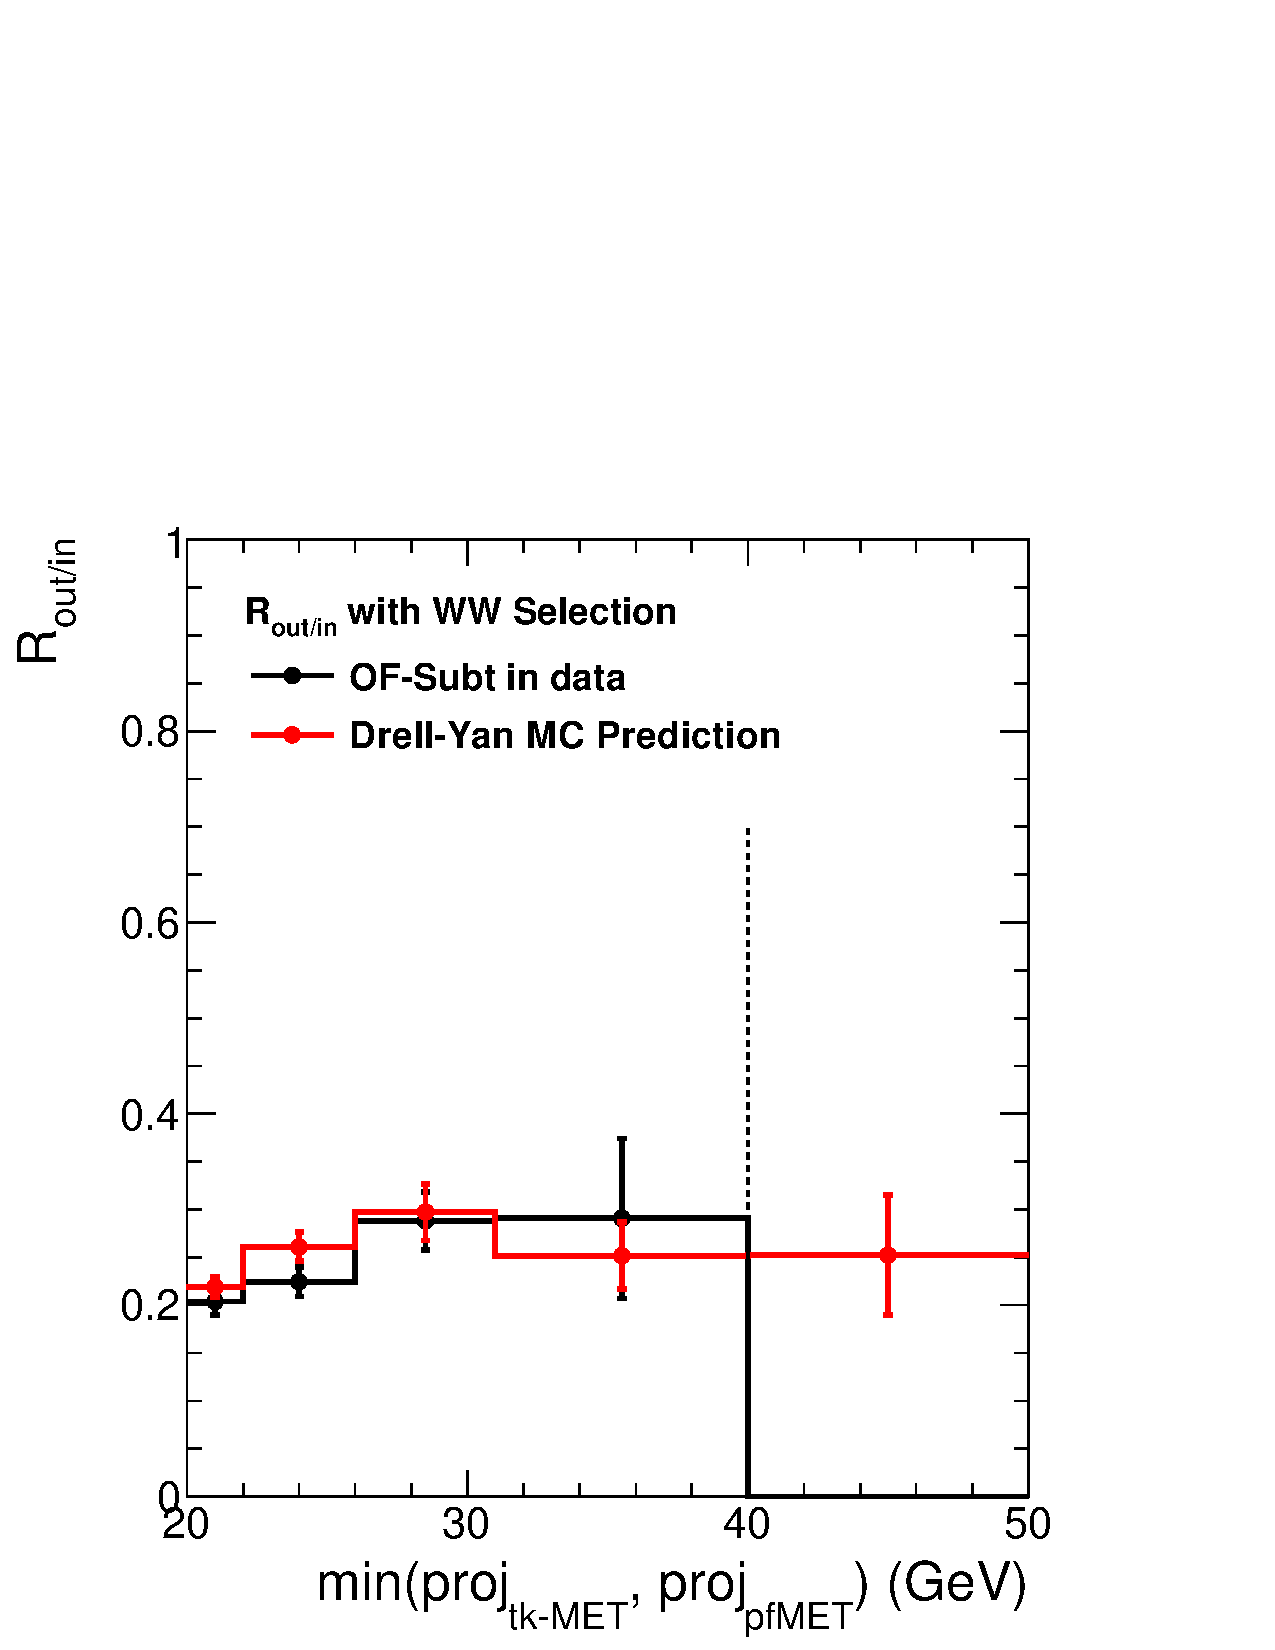
\includegraphics[width=.25\textwidth]{figures/Routin_0Jet_mH0_1092pb_dy.pdf} &
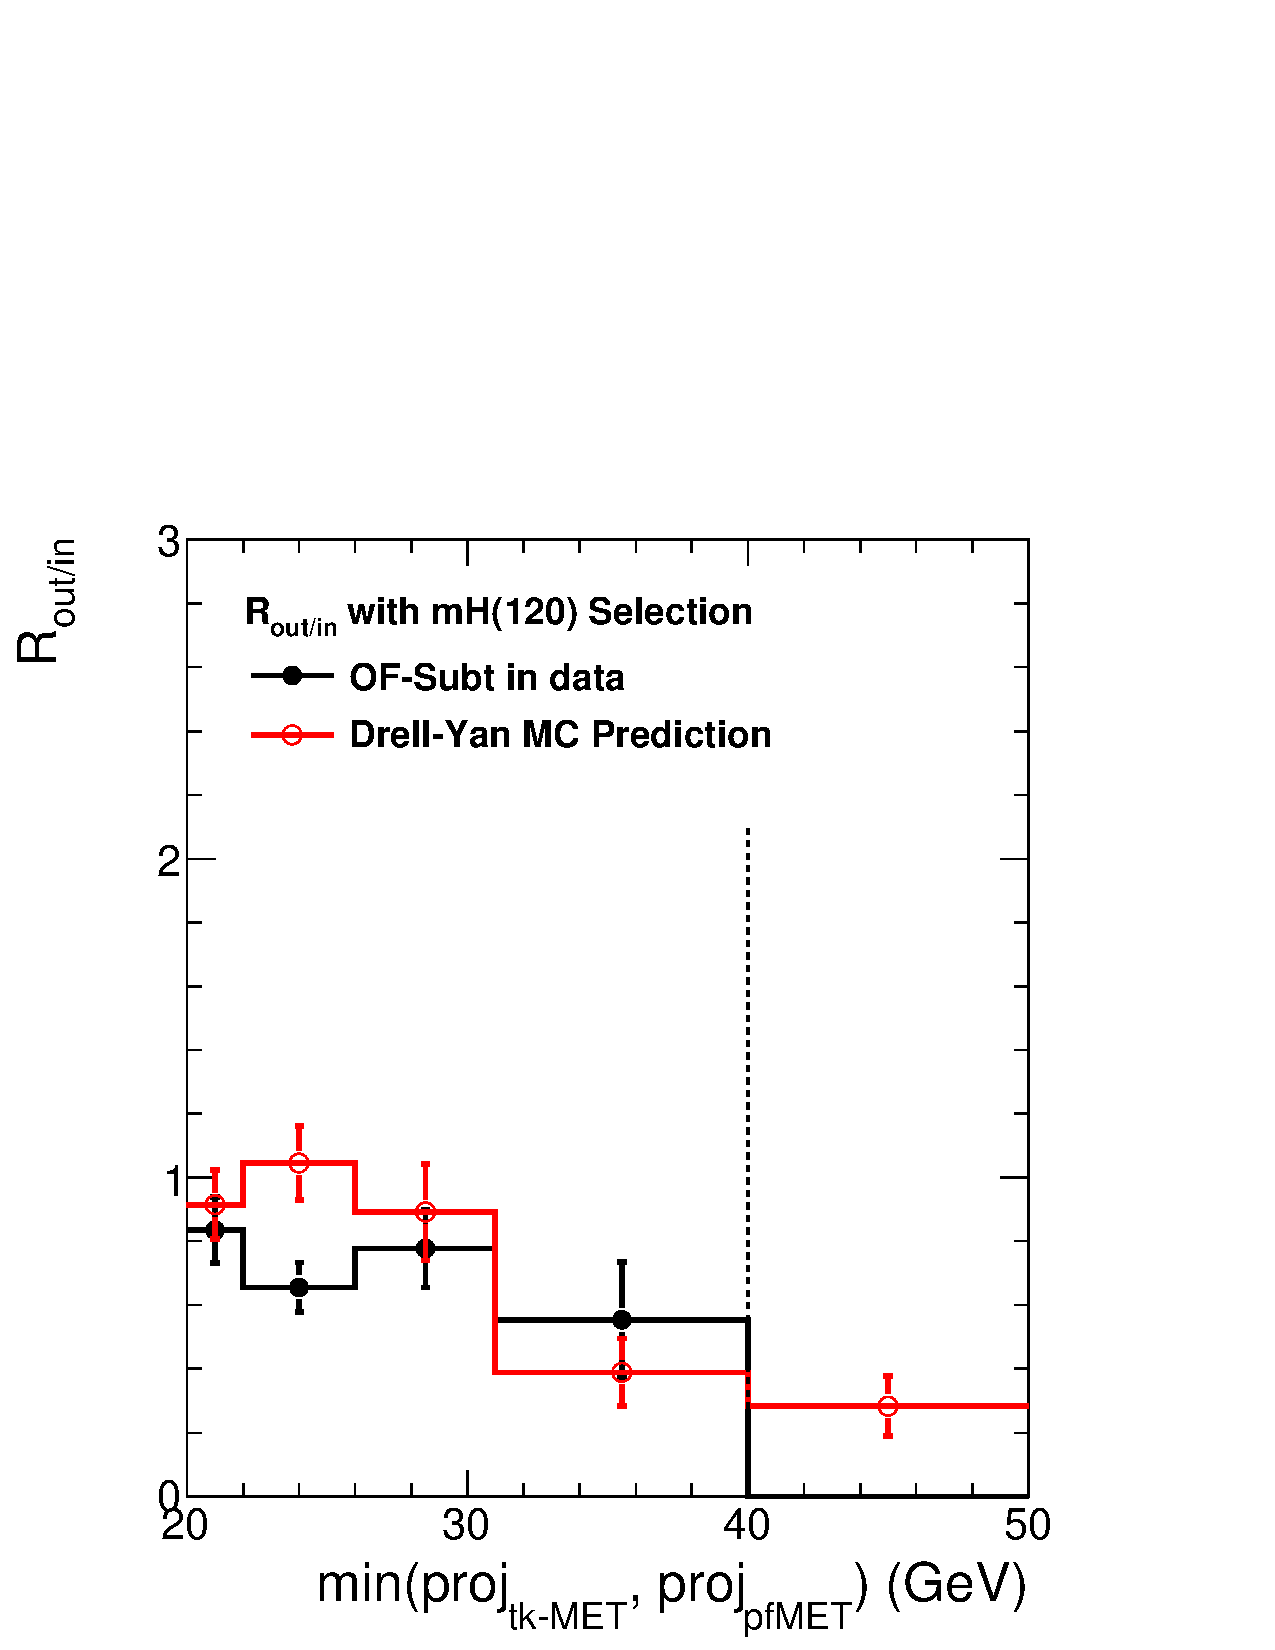
\includegraphics[width=.25\textwidth]{figures/Routin_0Jet_mH120_1092pb_dy.pdf} & 
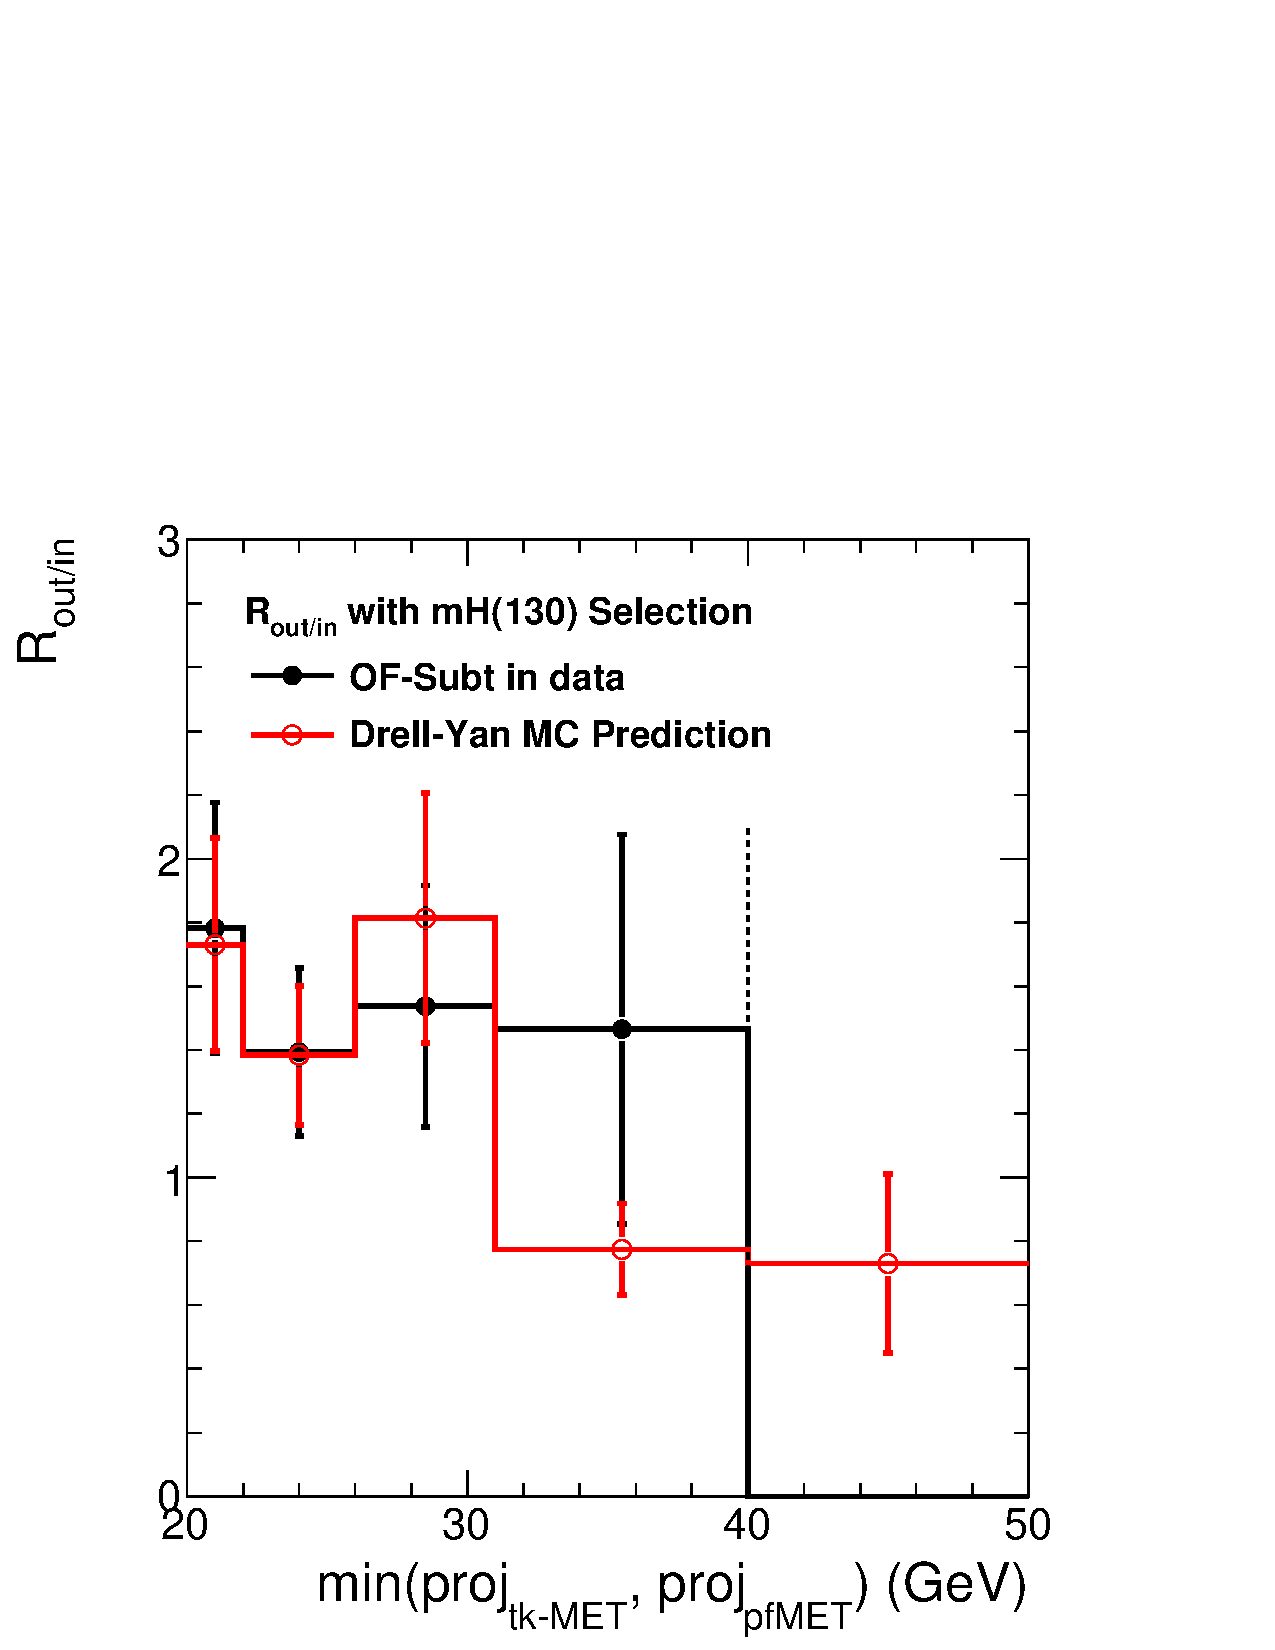
\includegraphics[width=.25\textwidth]{figures/Routin_0Jet_mH130_1092pb_dy.pdf} &
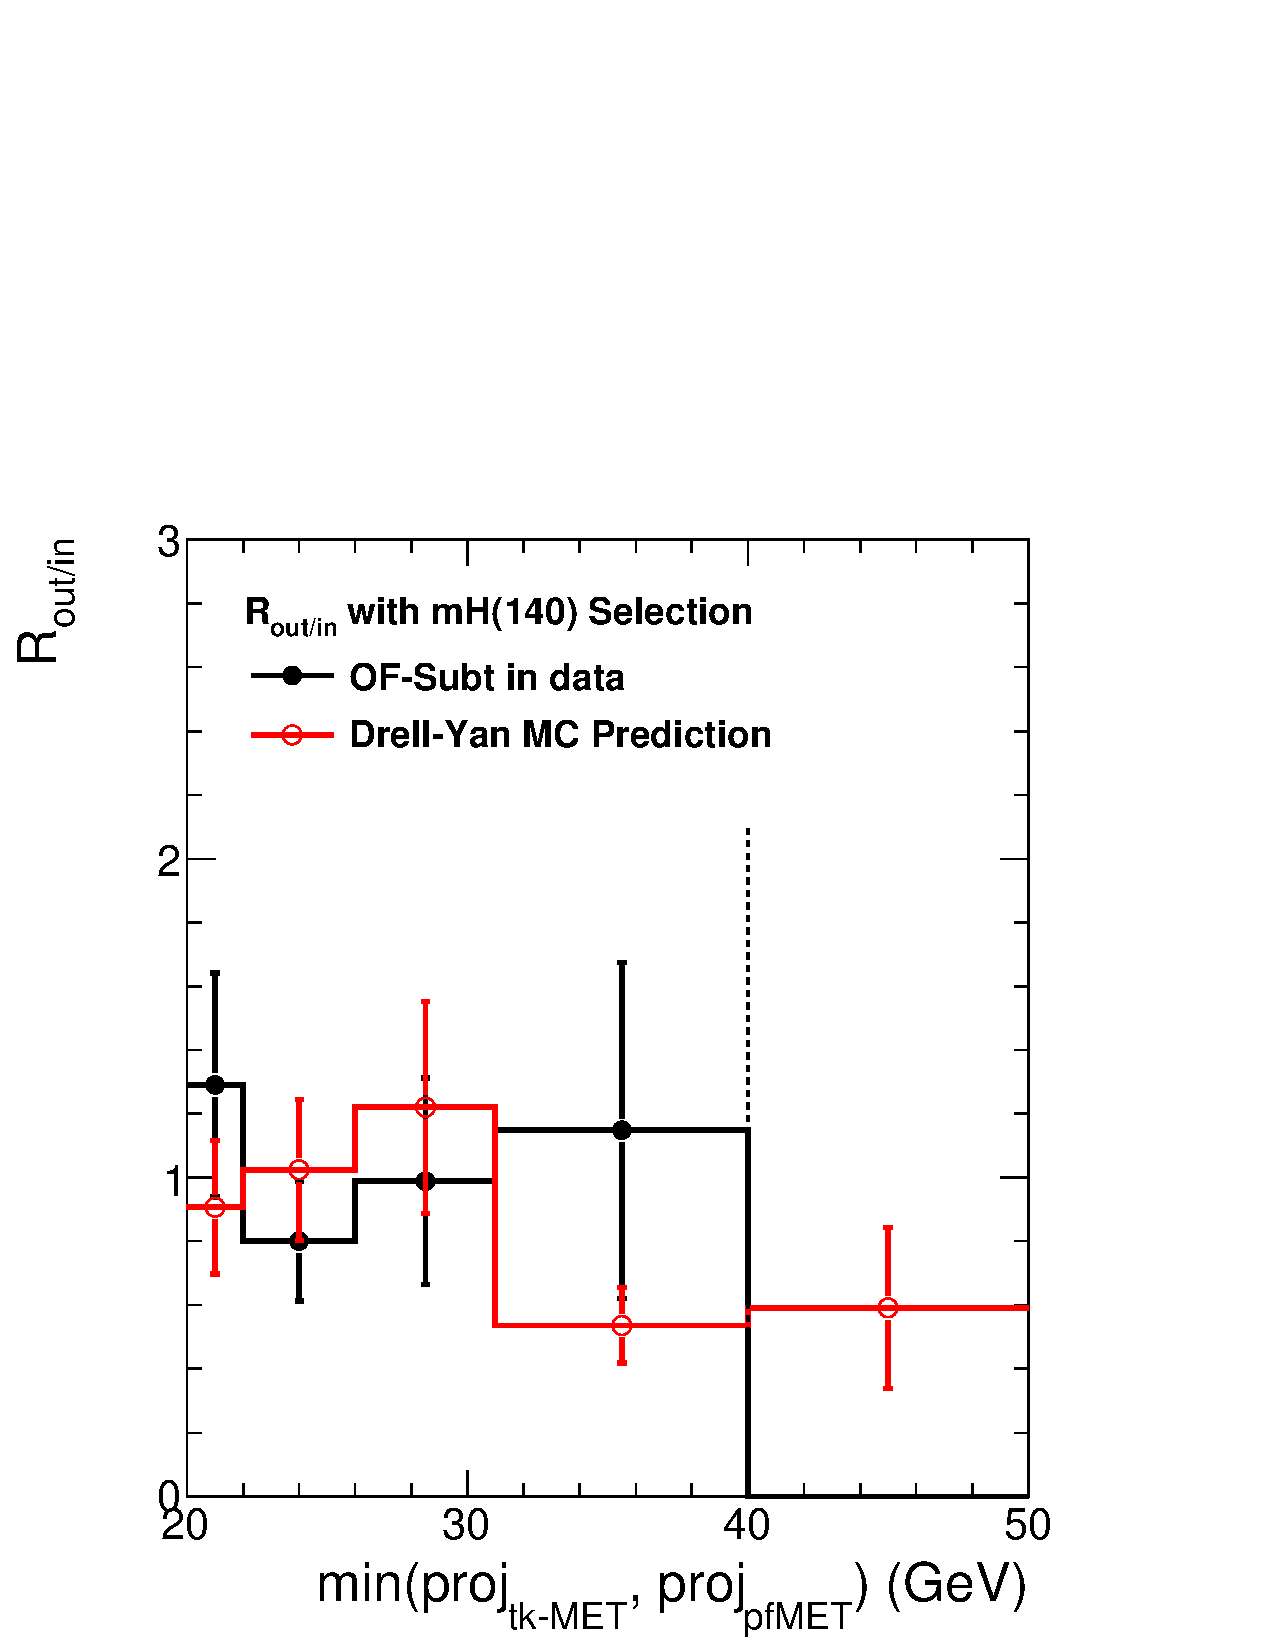
\includegraphics[width=.25\textwidth]{figures/Routin_0Jet_mH140_1092pb_dy.pdf} \\
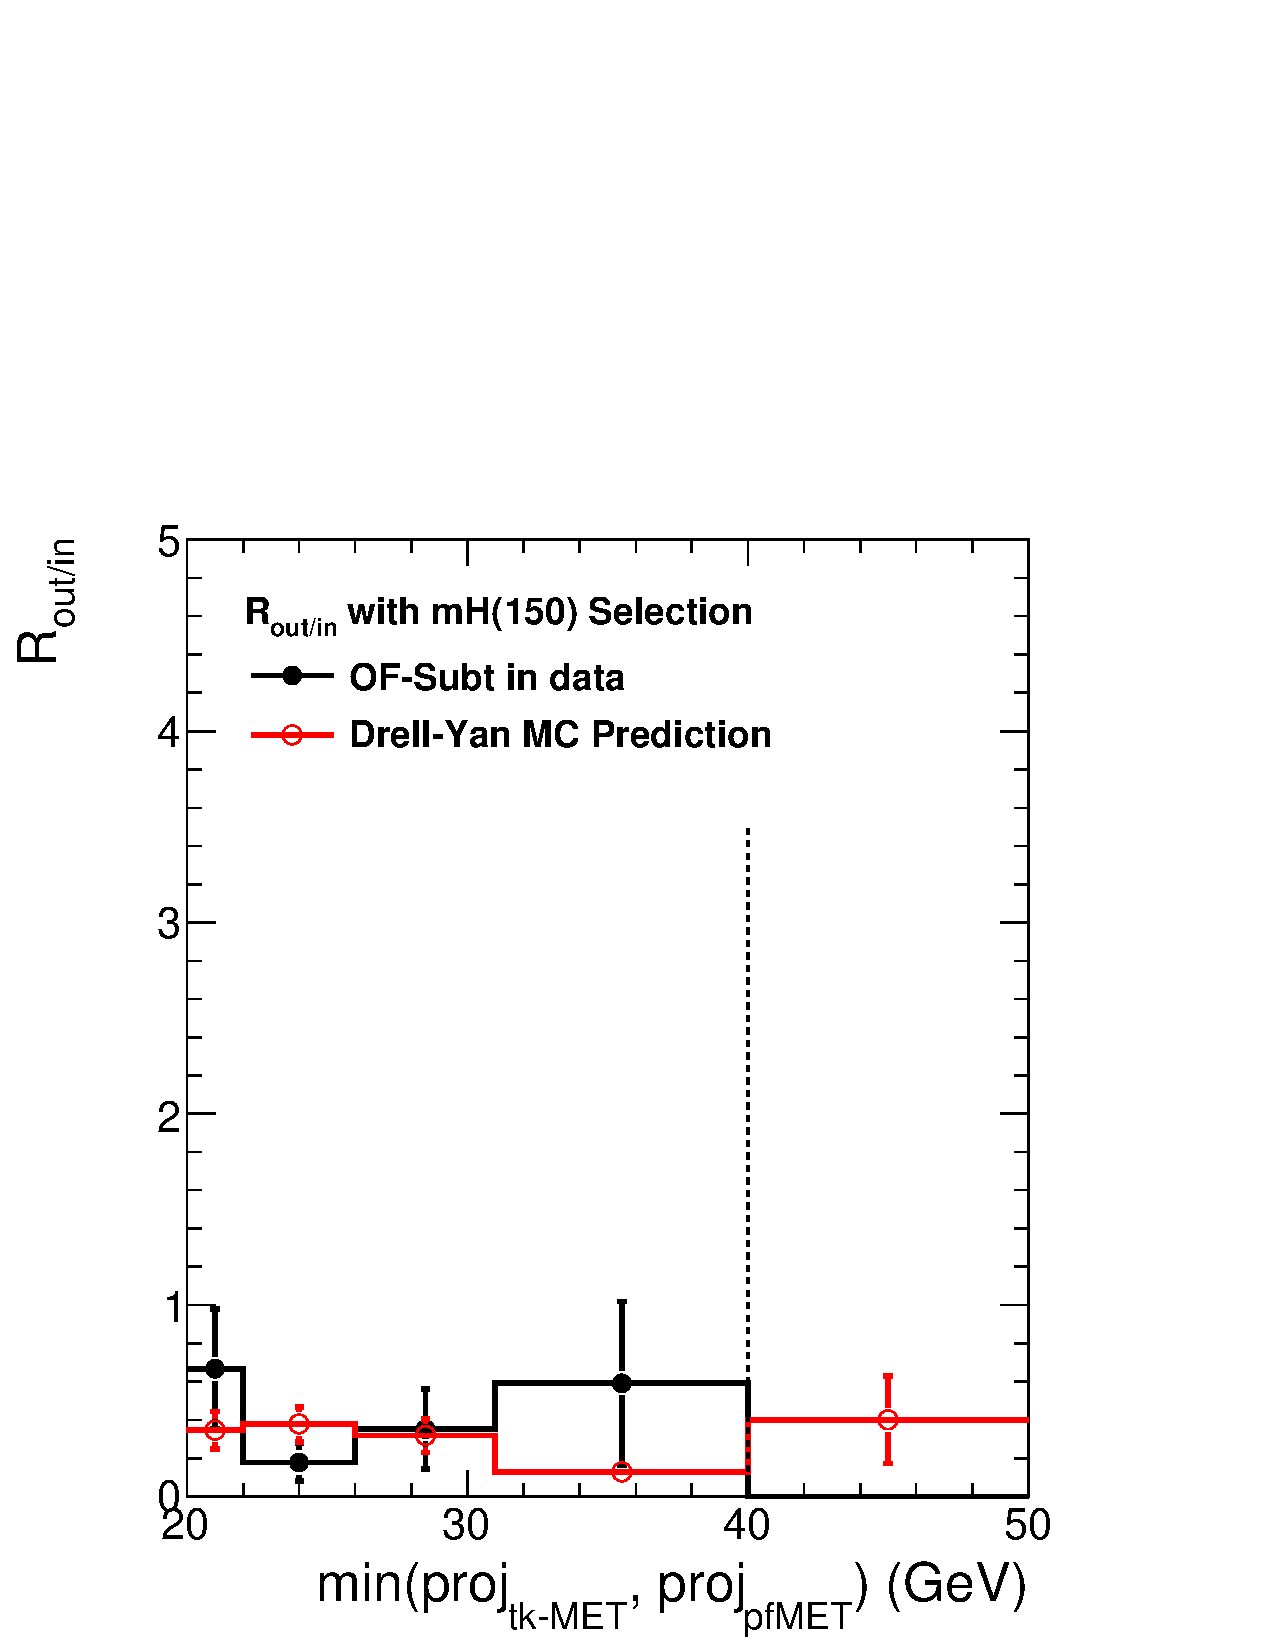
\includegraphics[width=.25\textwidth]{figures/Routin_0Jet_mH150_1092pb_dy.pdf} &
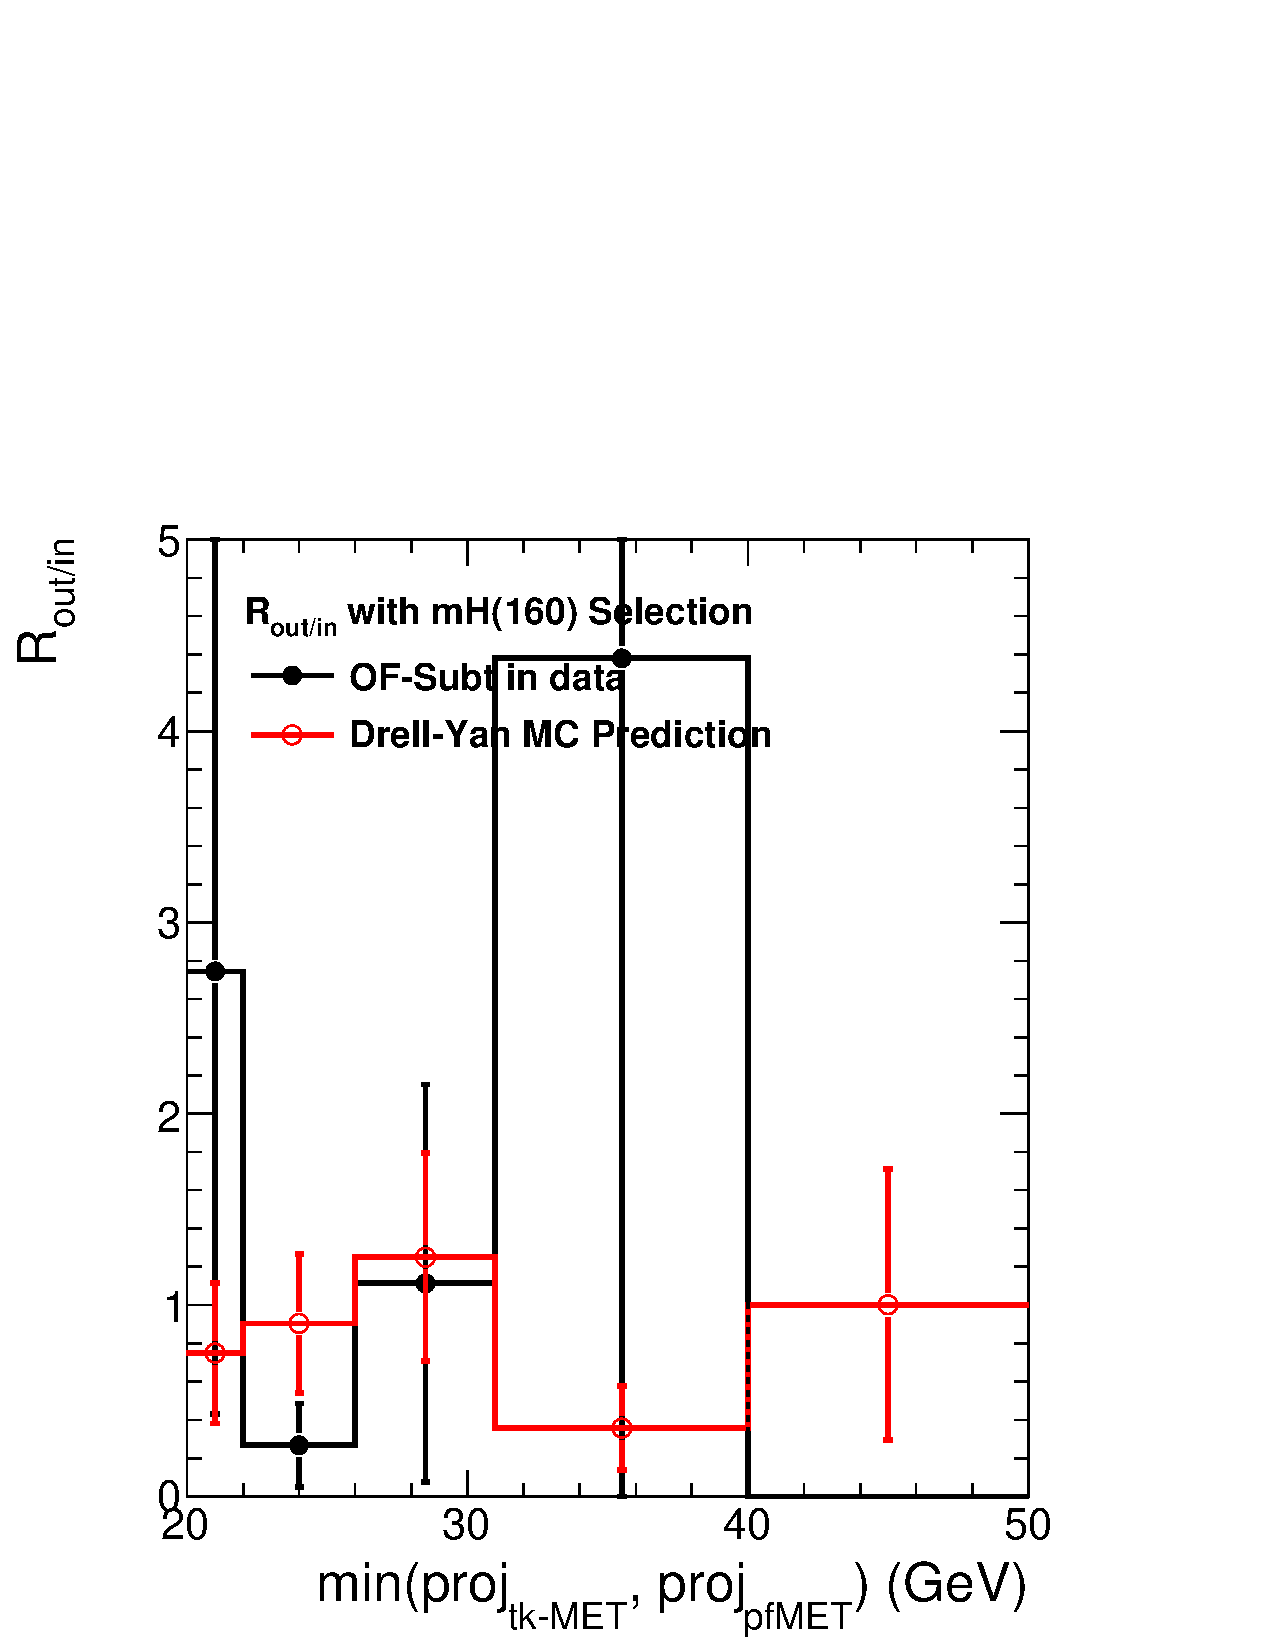
\includegraphics[width=.25\textwidth]{figures/Routin_0Jet_mH160_1092pb_dy.pdf} &
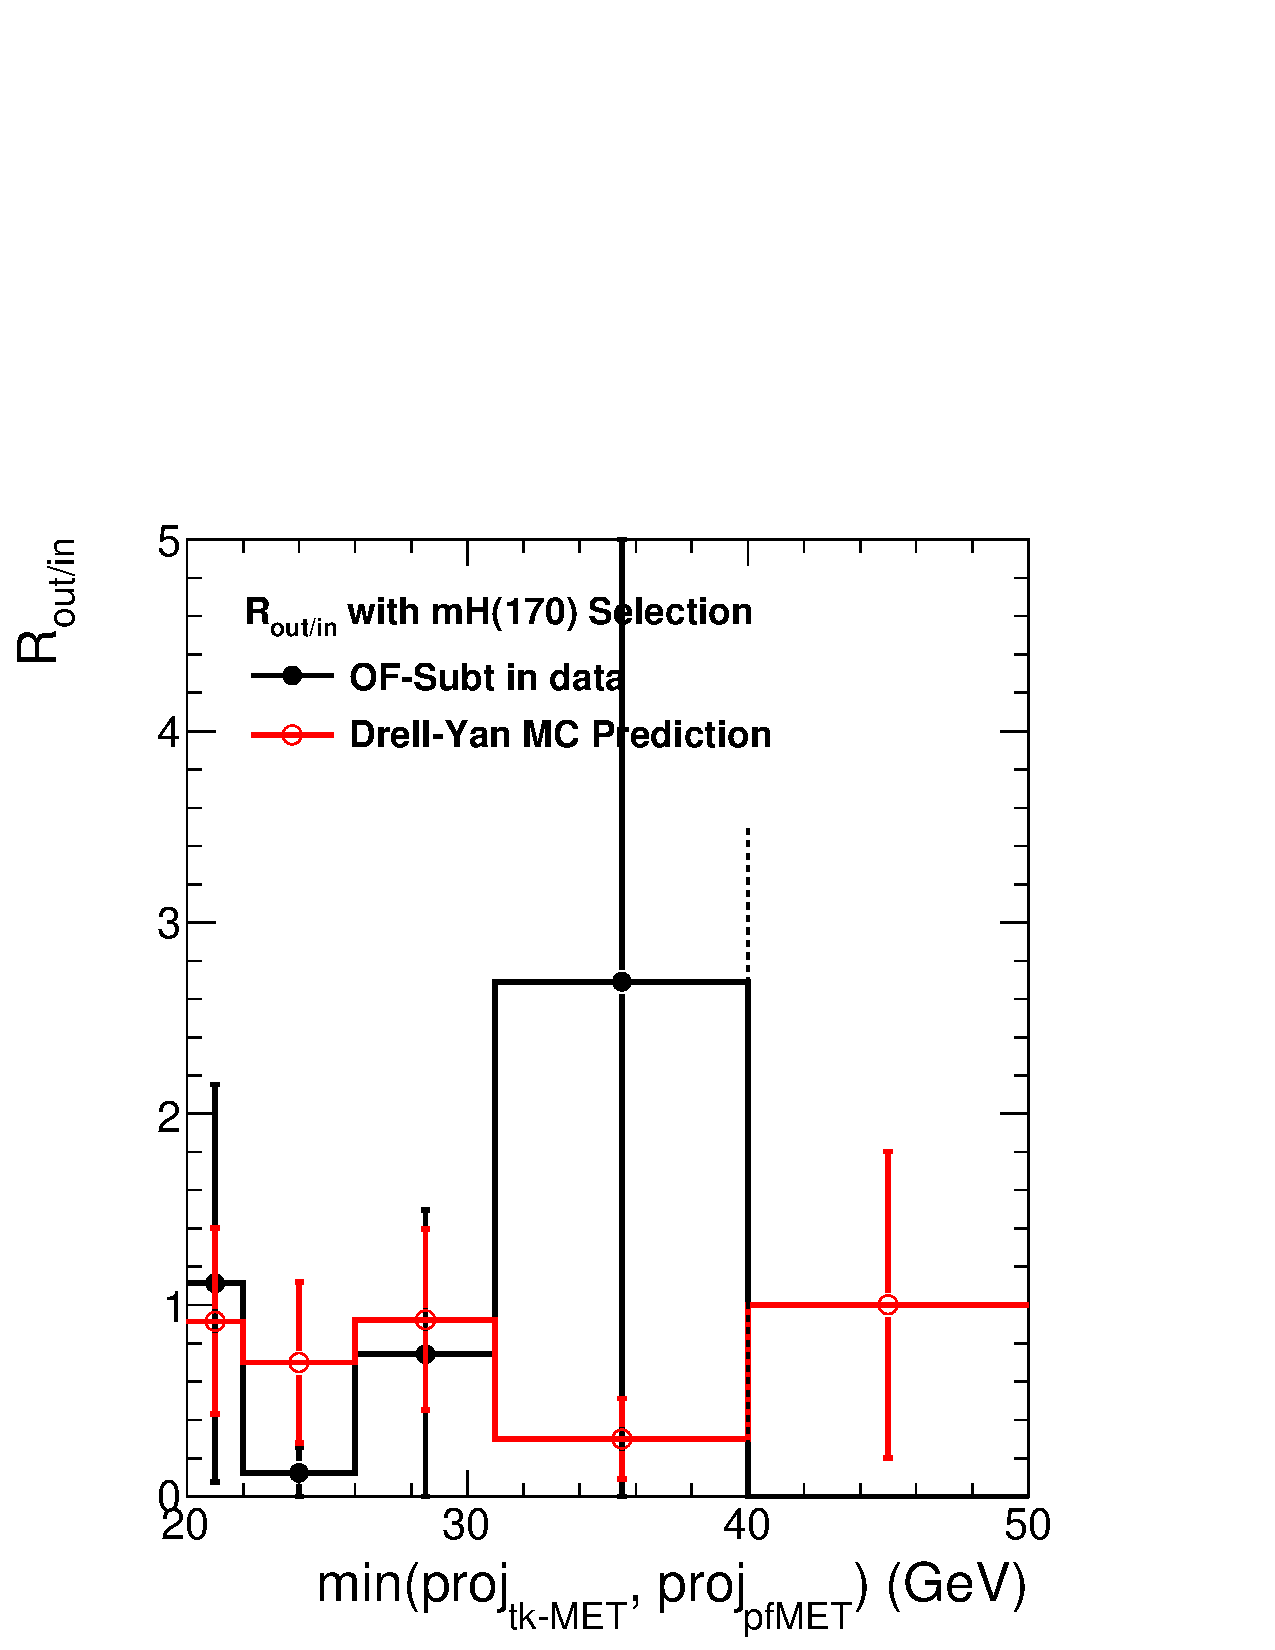
\includegraphics[width=.25\textwidth]{figures/Routin_0Jet_mH170_1092pb_dy.pdf} &
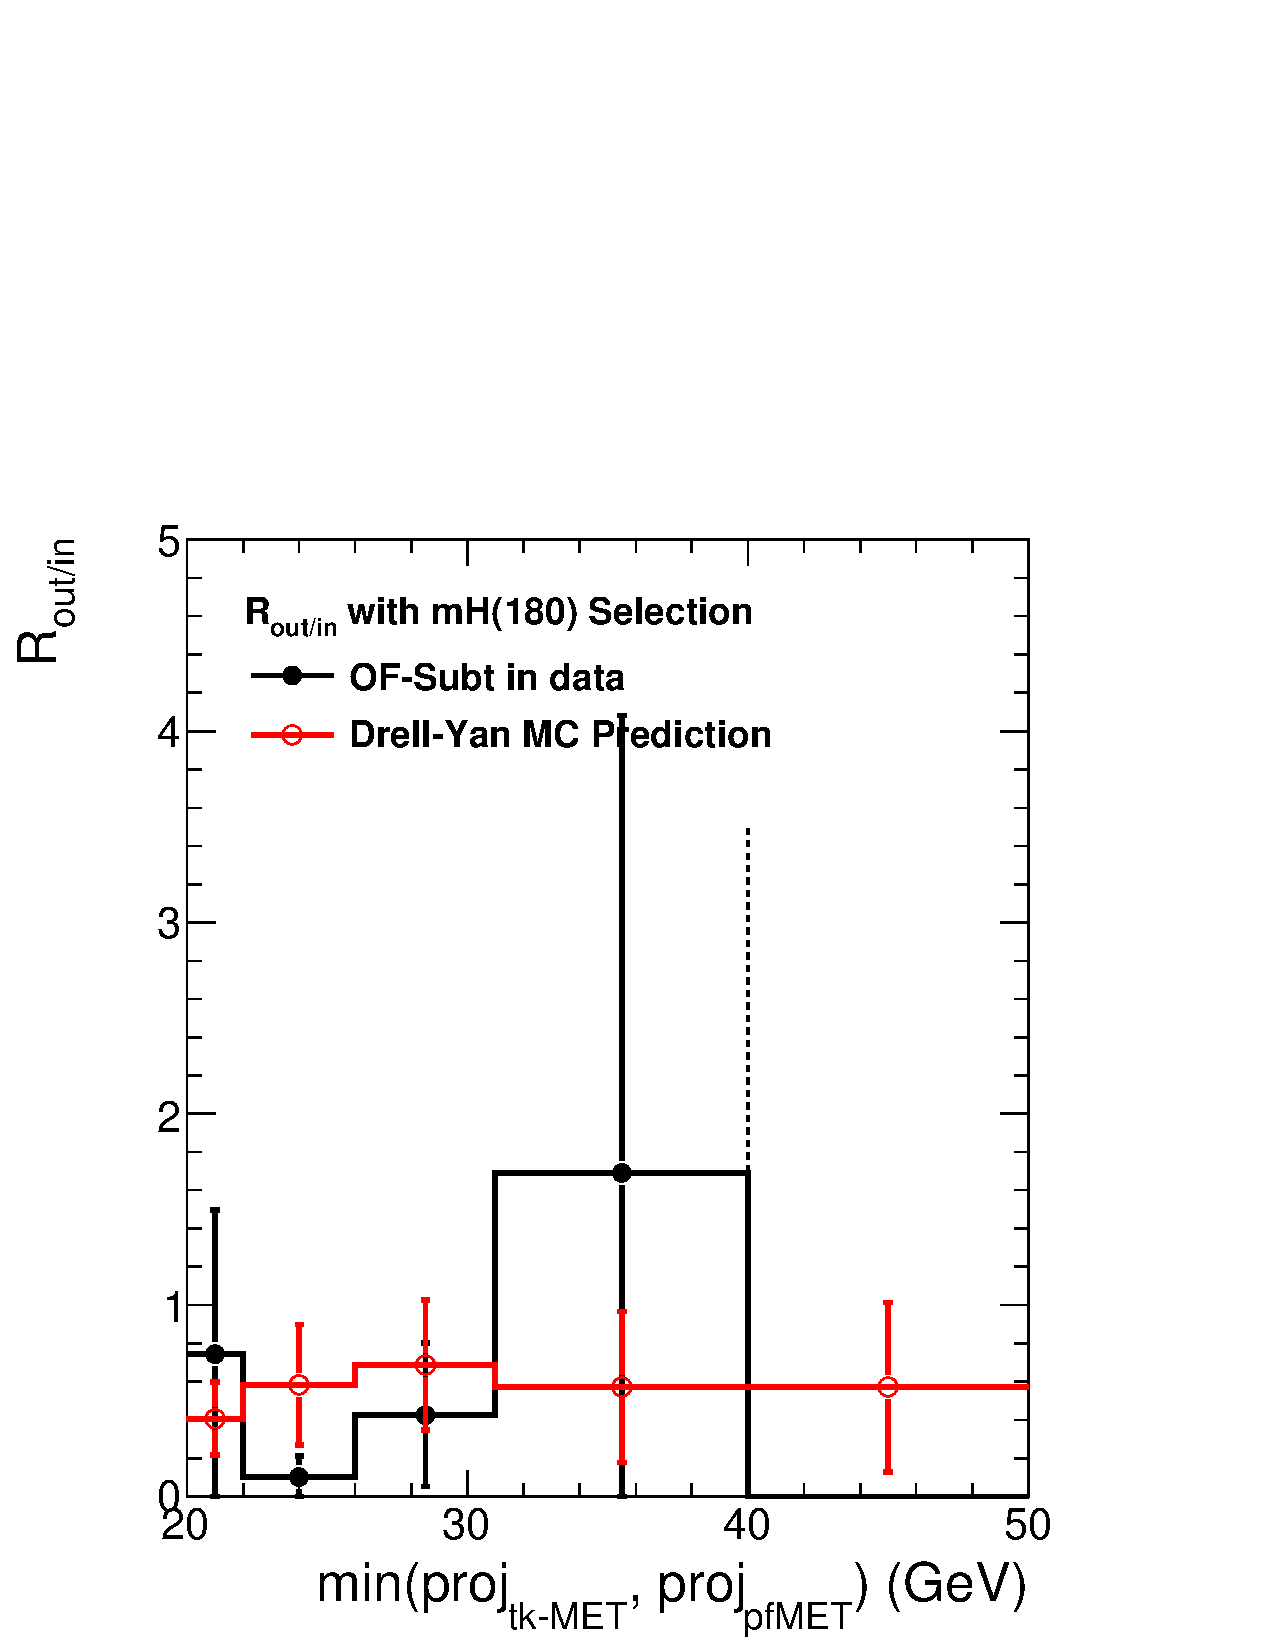
\includegraphics[width=.25\textwidth]{figures/Routin_0Jet_mH180_1092pb_dy.pdf} \\
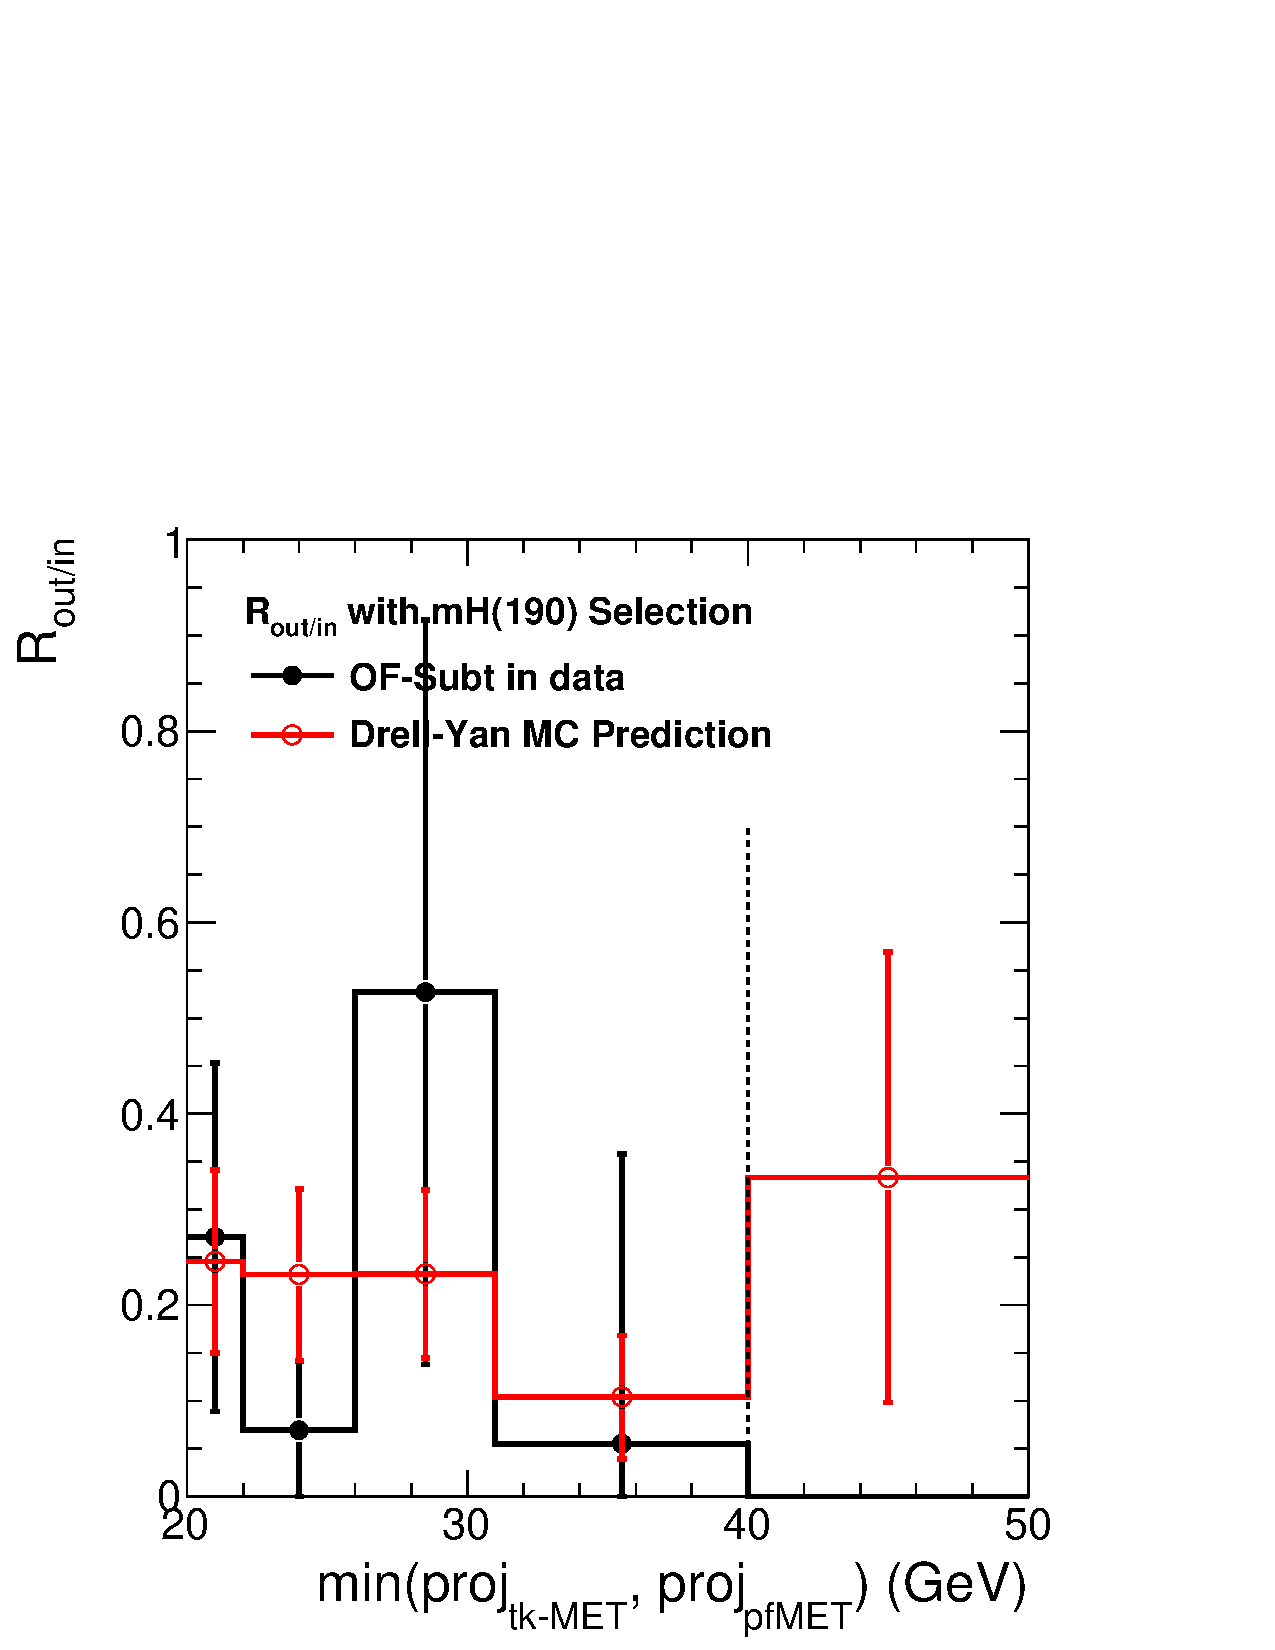
\includegraphics[width=.25\textwidth]{figures/Routin_0Jet_mH190_1092pb_dy.pdf} &
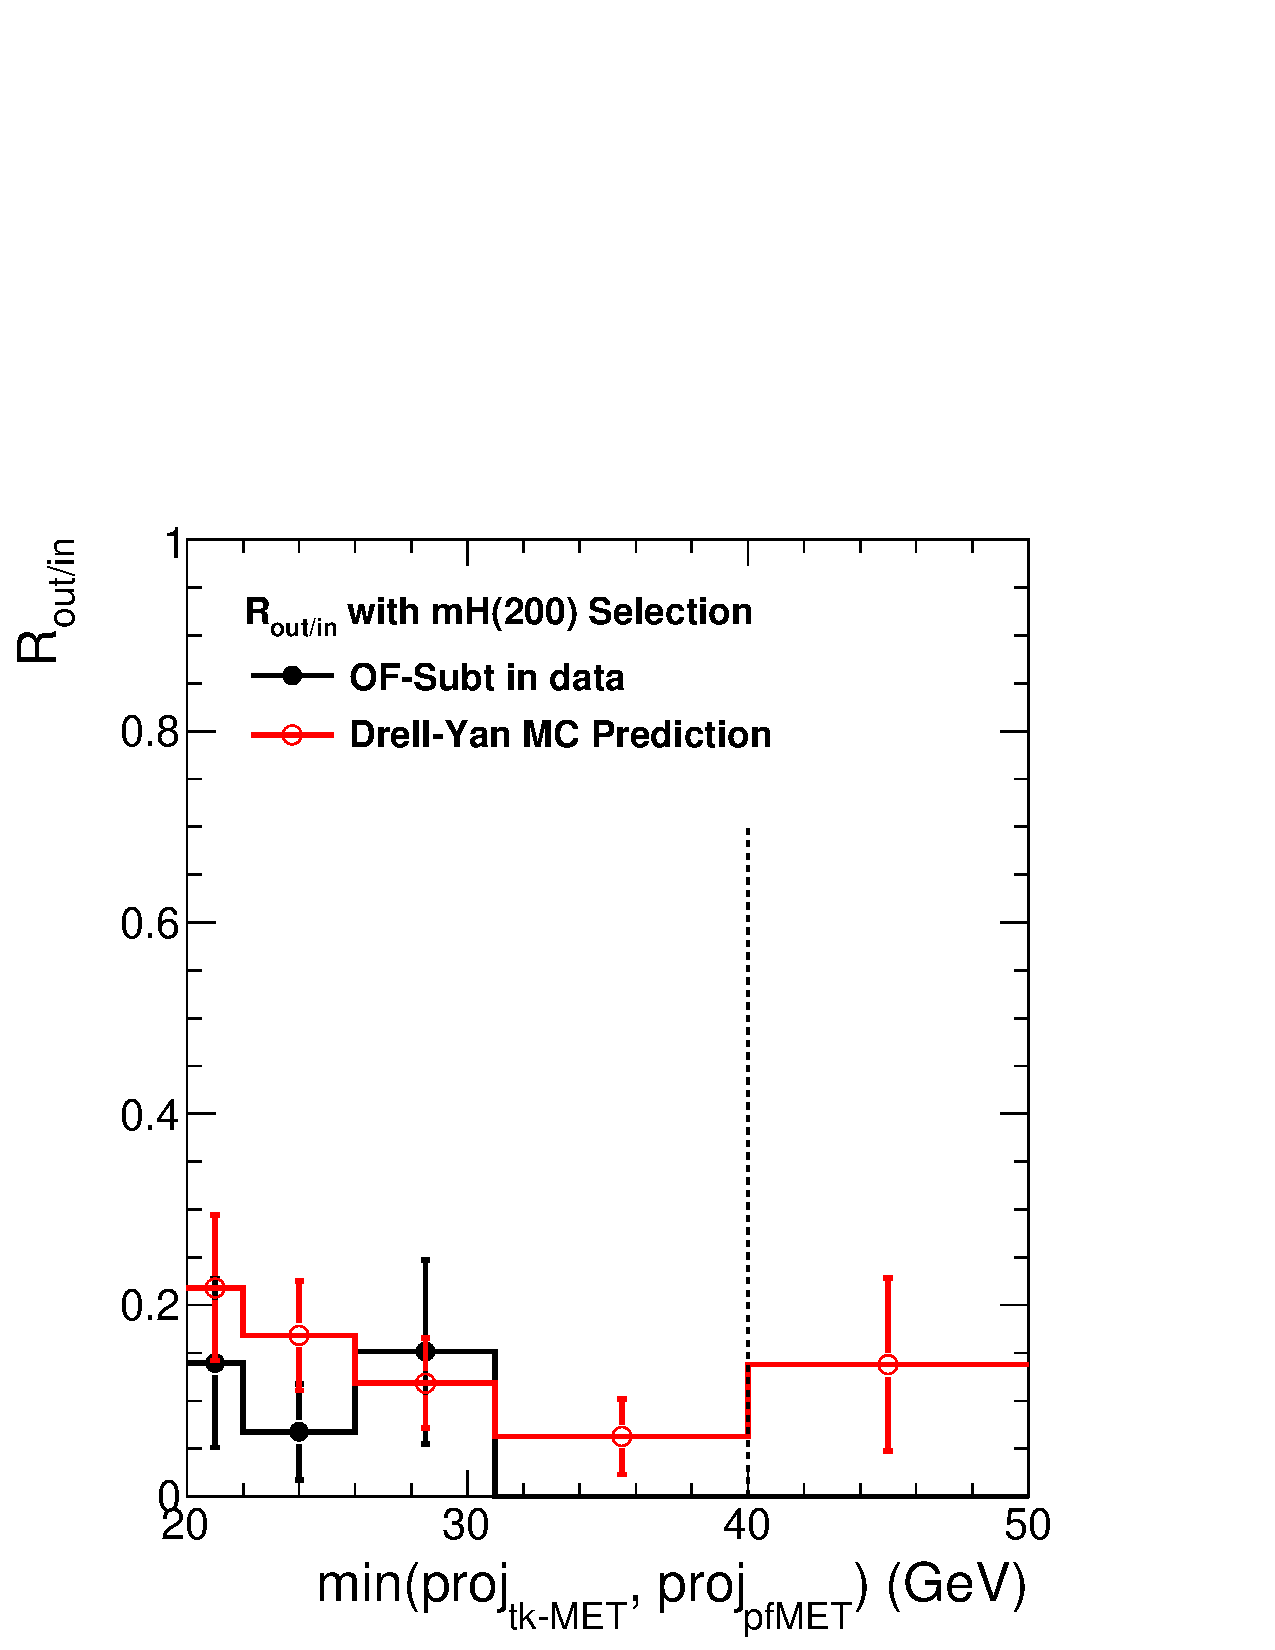
\includegraphics[width=.25\textwidth]{figures/Routin_0Jet_mH200_1092pb_dy.pdf} &
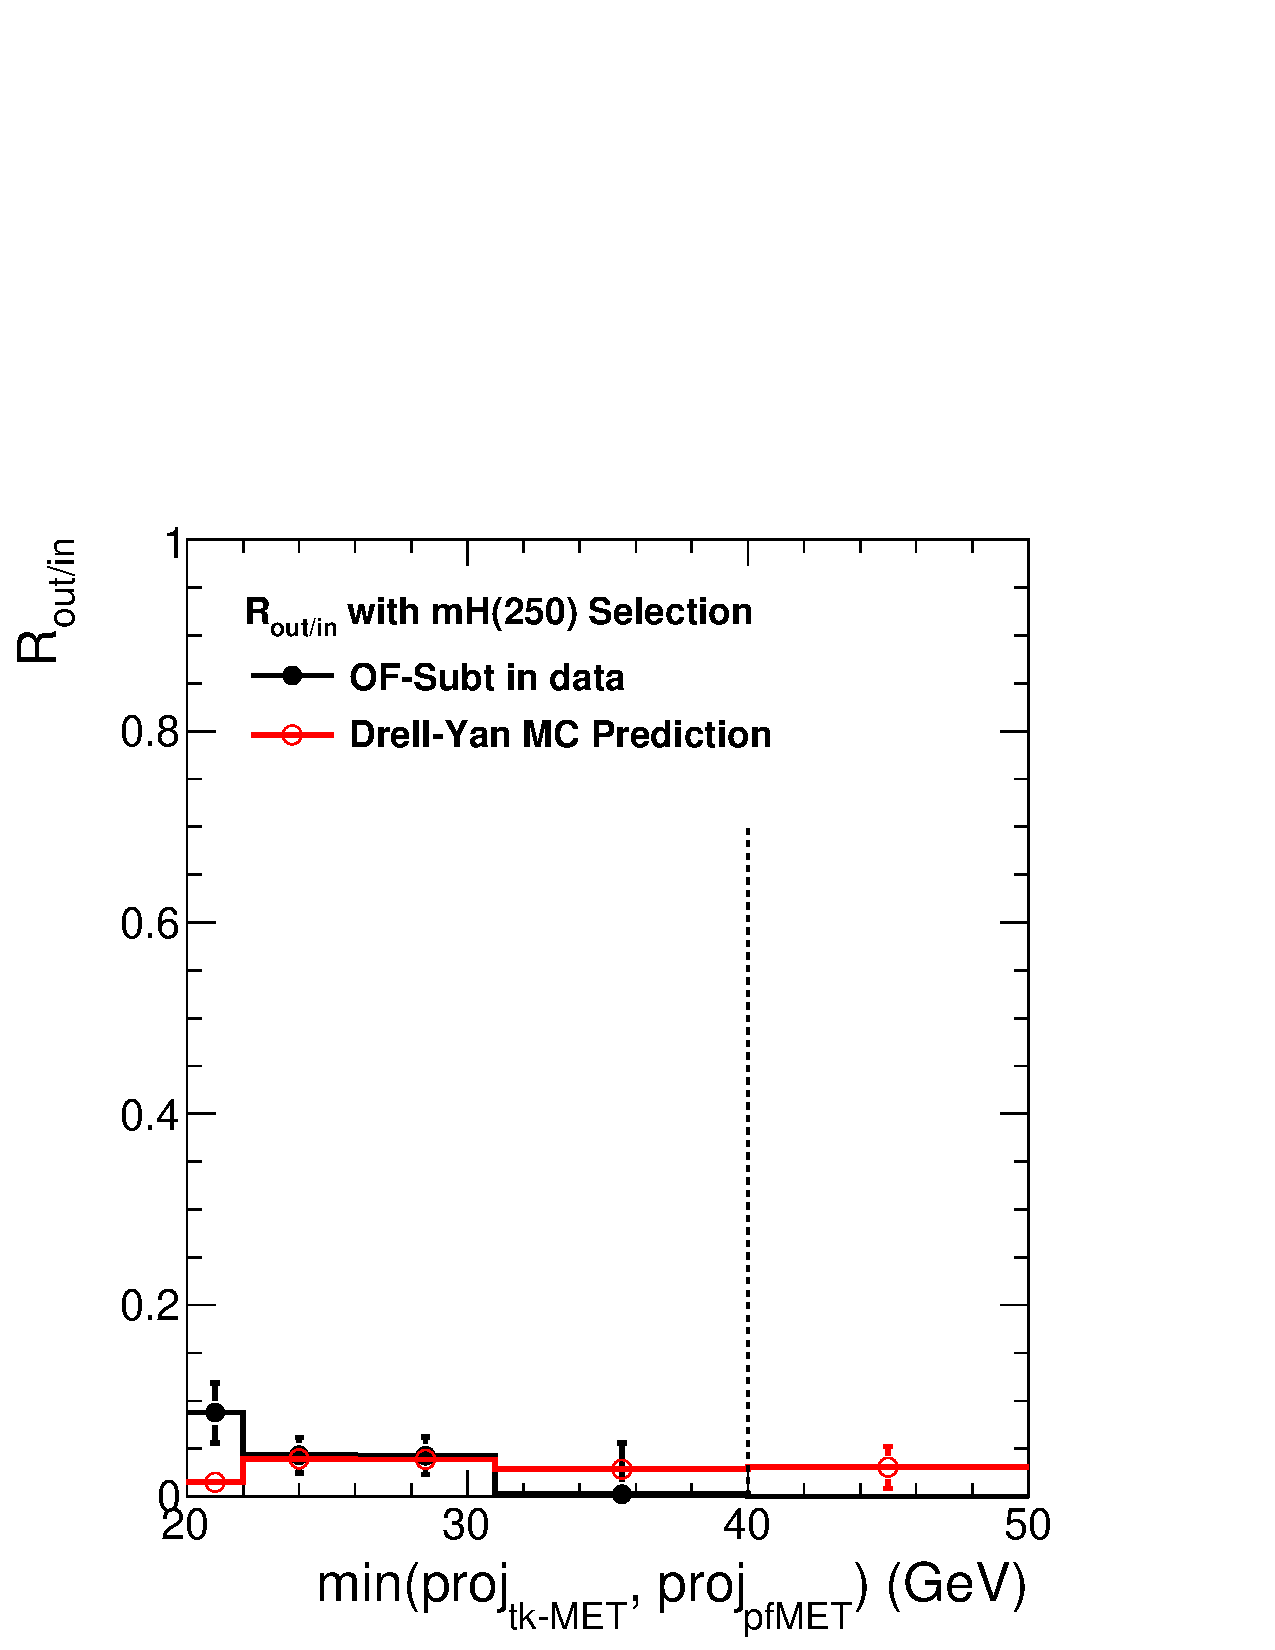
\includegraphics[width=.25\textwidth]{figures/Routin_0Jet_mH250_1092pb_dy.pdf} &
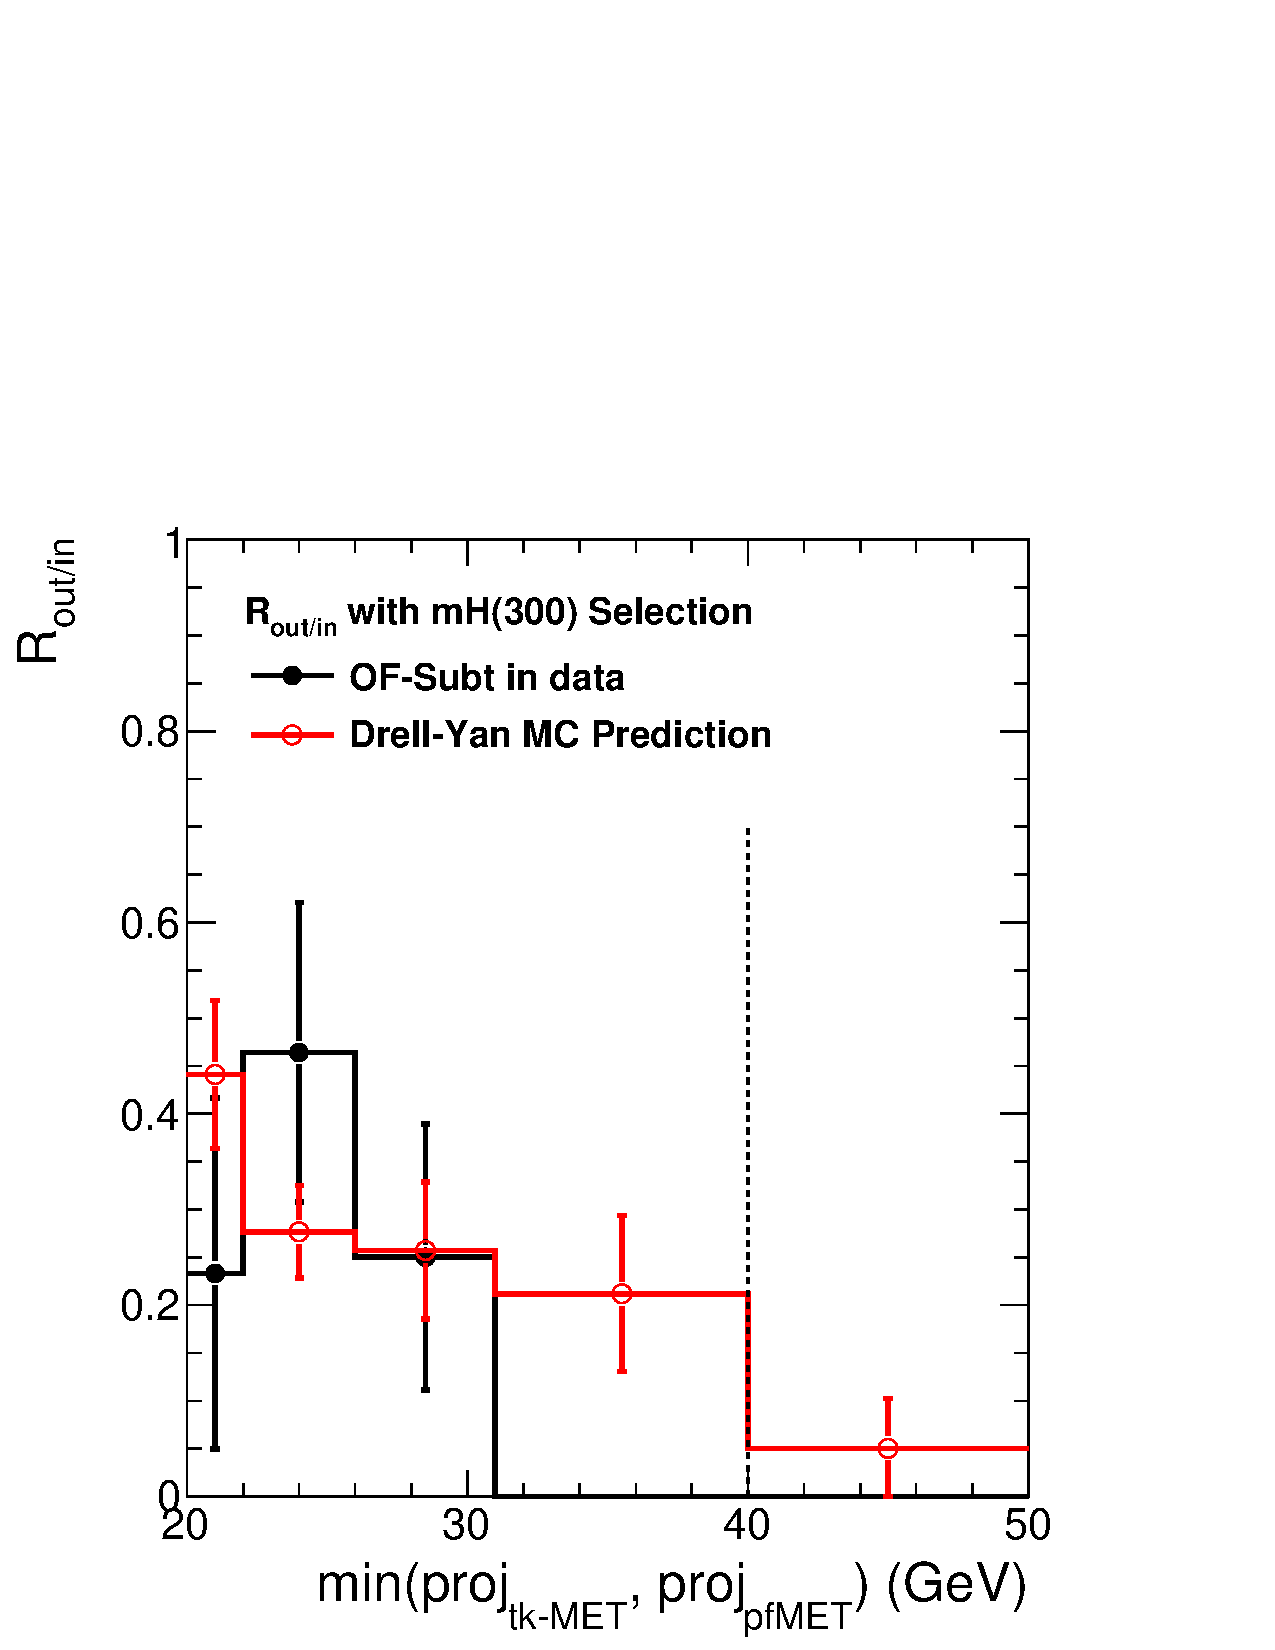
\includegraphics[width=.25\textwidth]{figures/Routin_0Jet_mH300_1092pb_dy.pdf} \\
\end{array}$
\caption{ The \routin\, as a function of MET measured from data (black solid dots) 
and MC (red open circles) for the Drell-Yan processes in the 0-Jet bin. 
The measurements in data are performed in the control region where we select events 
with MET less than the 40 GeV (black dashed line) using the opposite flavor subtraction method. 
The MC measurements extend into the signal region shown in the last bin. 
The difference in the \routin measurements in different higg selections are due to the 
different kinematic cuts applied. 
}
\label{fig:routin_0jet}
\end{center}
\end{figure}

\begin{figure}[!htbp]
\begin{center}$
\begin{array}{cccc}
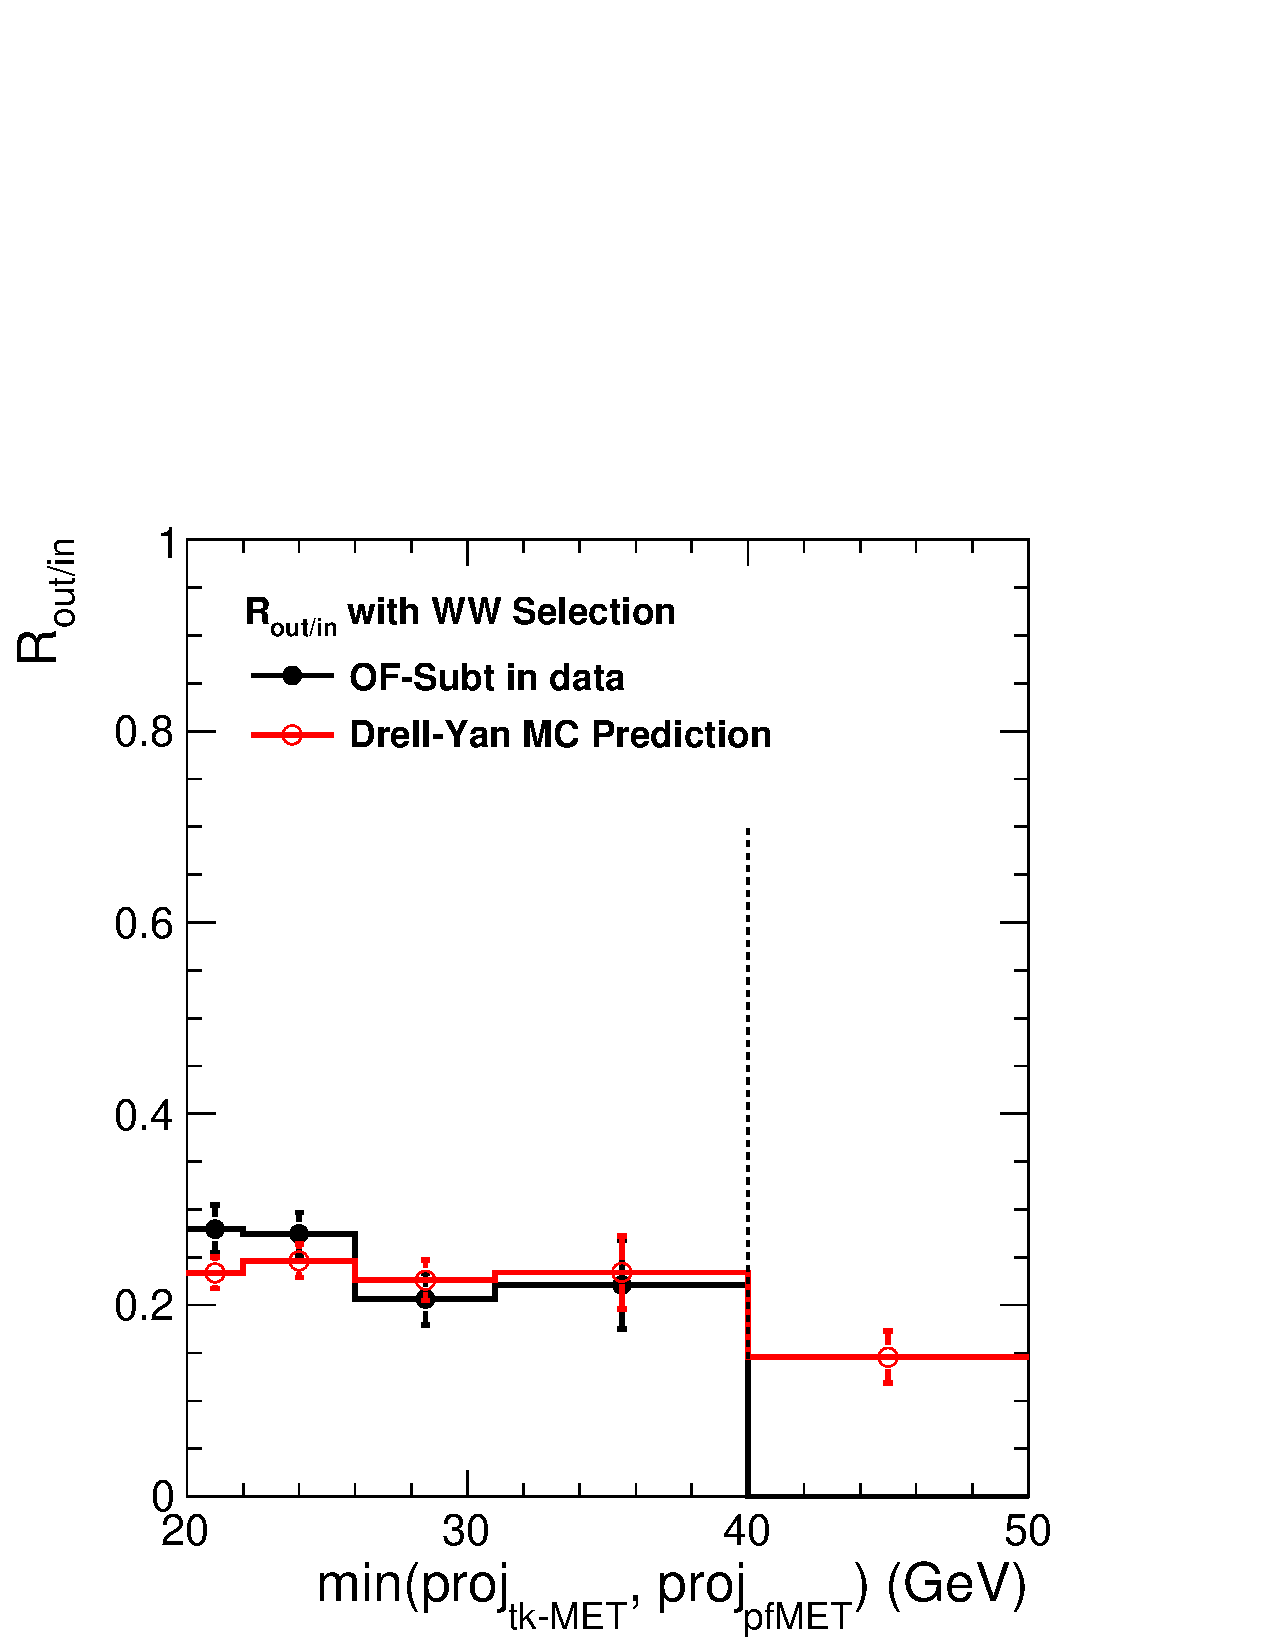
\includegraphics[width=.25\textwidth]{figures/Routin_1Jet_mH0_1092pb_dy.pdf}&
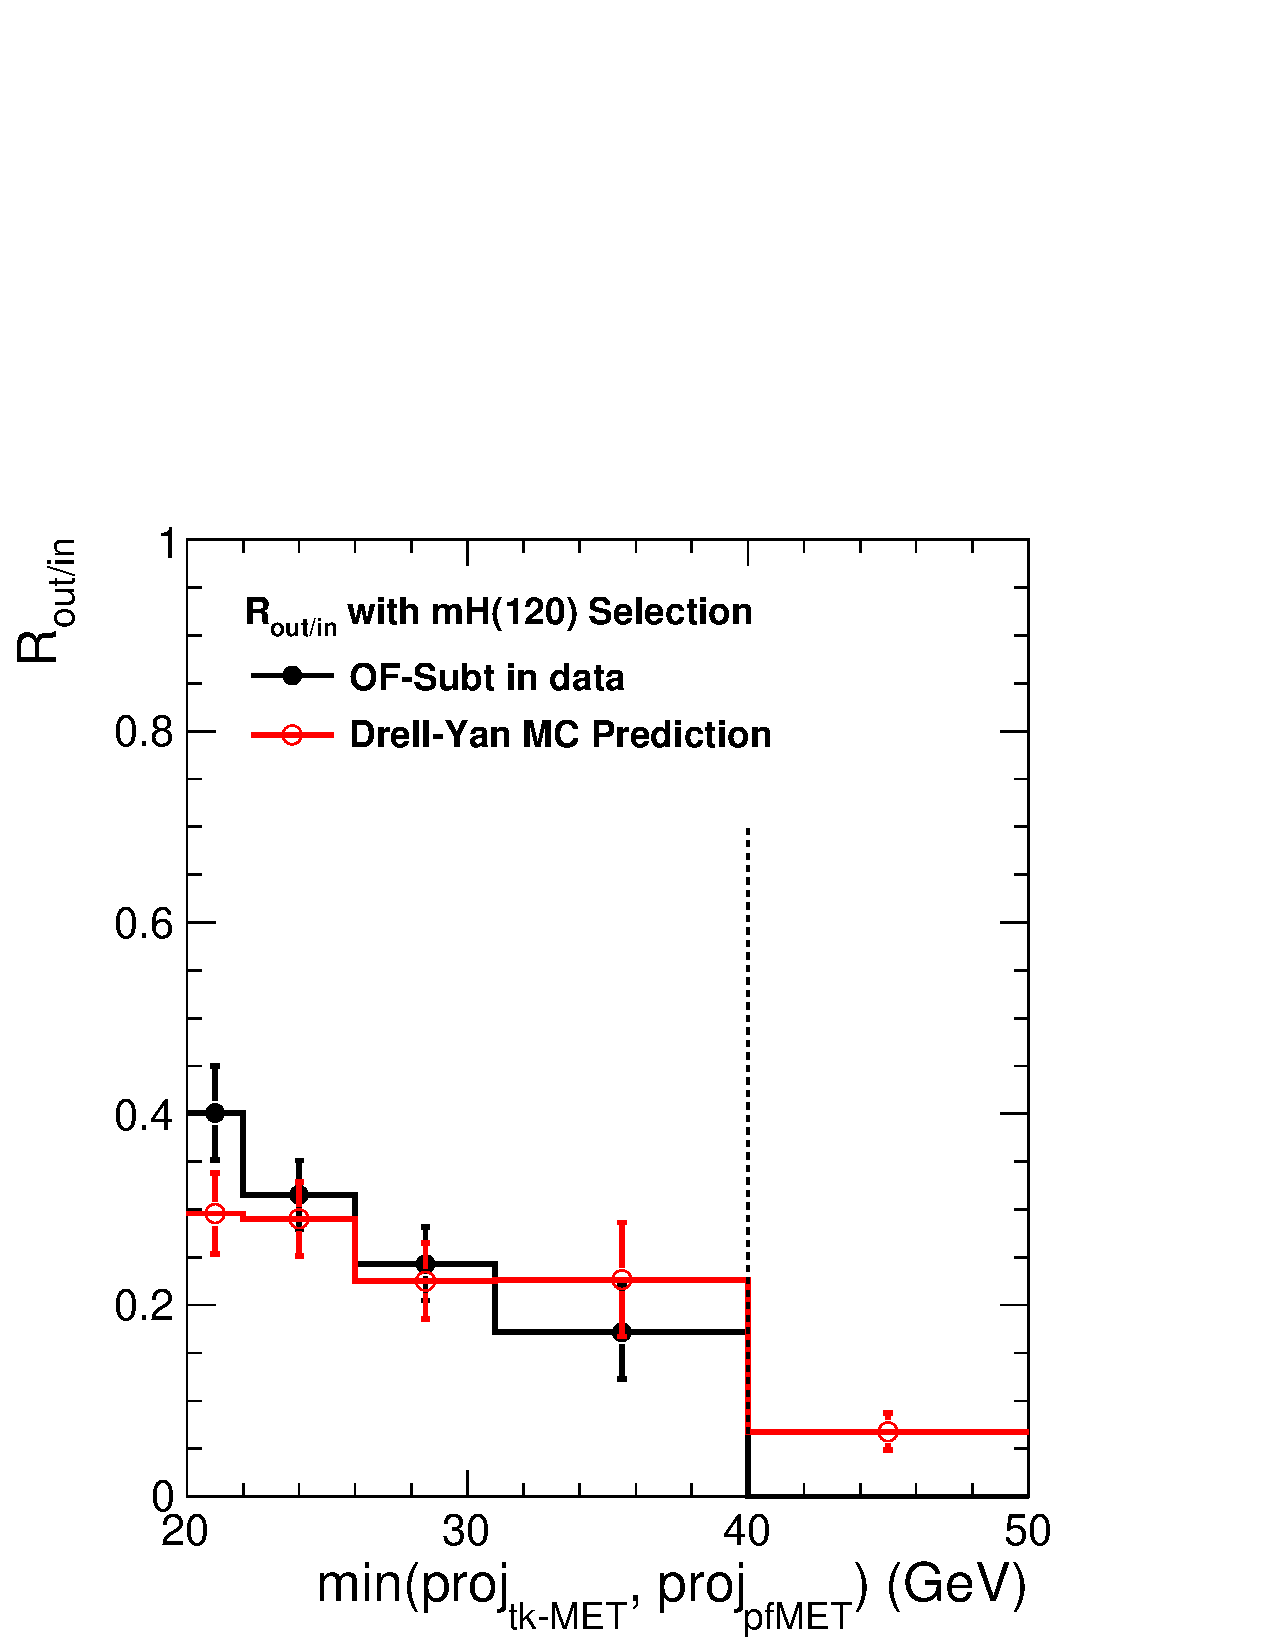
\includegraphics[width=.25\textwidth]{figures/Routin_1Jet_mH120_1092pb_dy.pdf}&
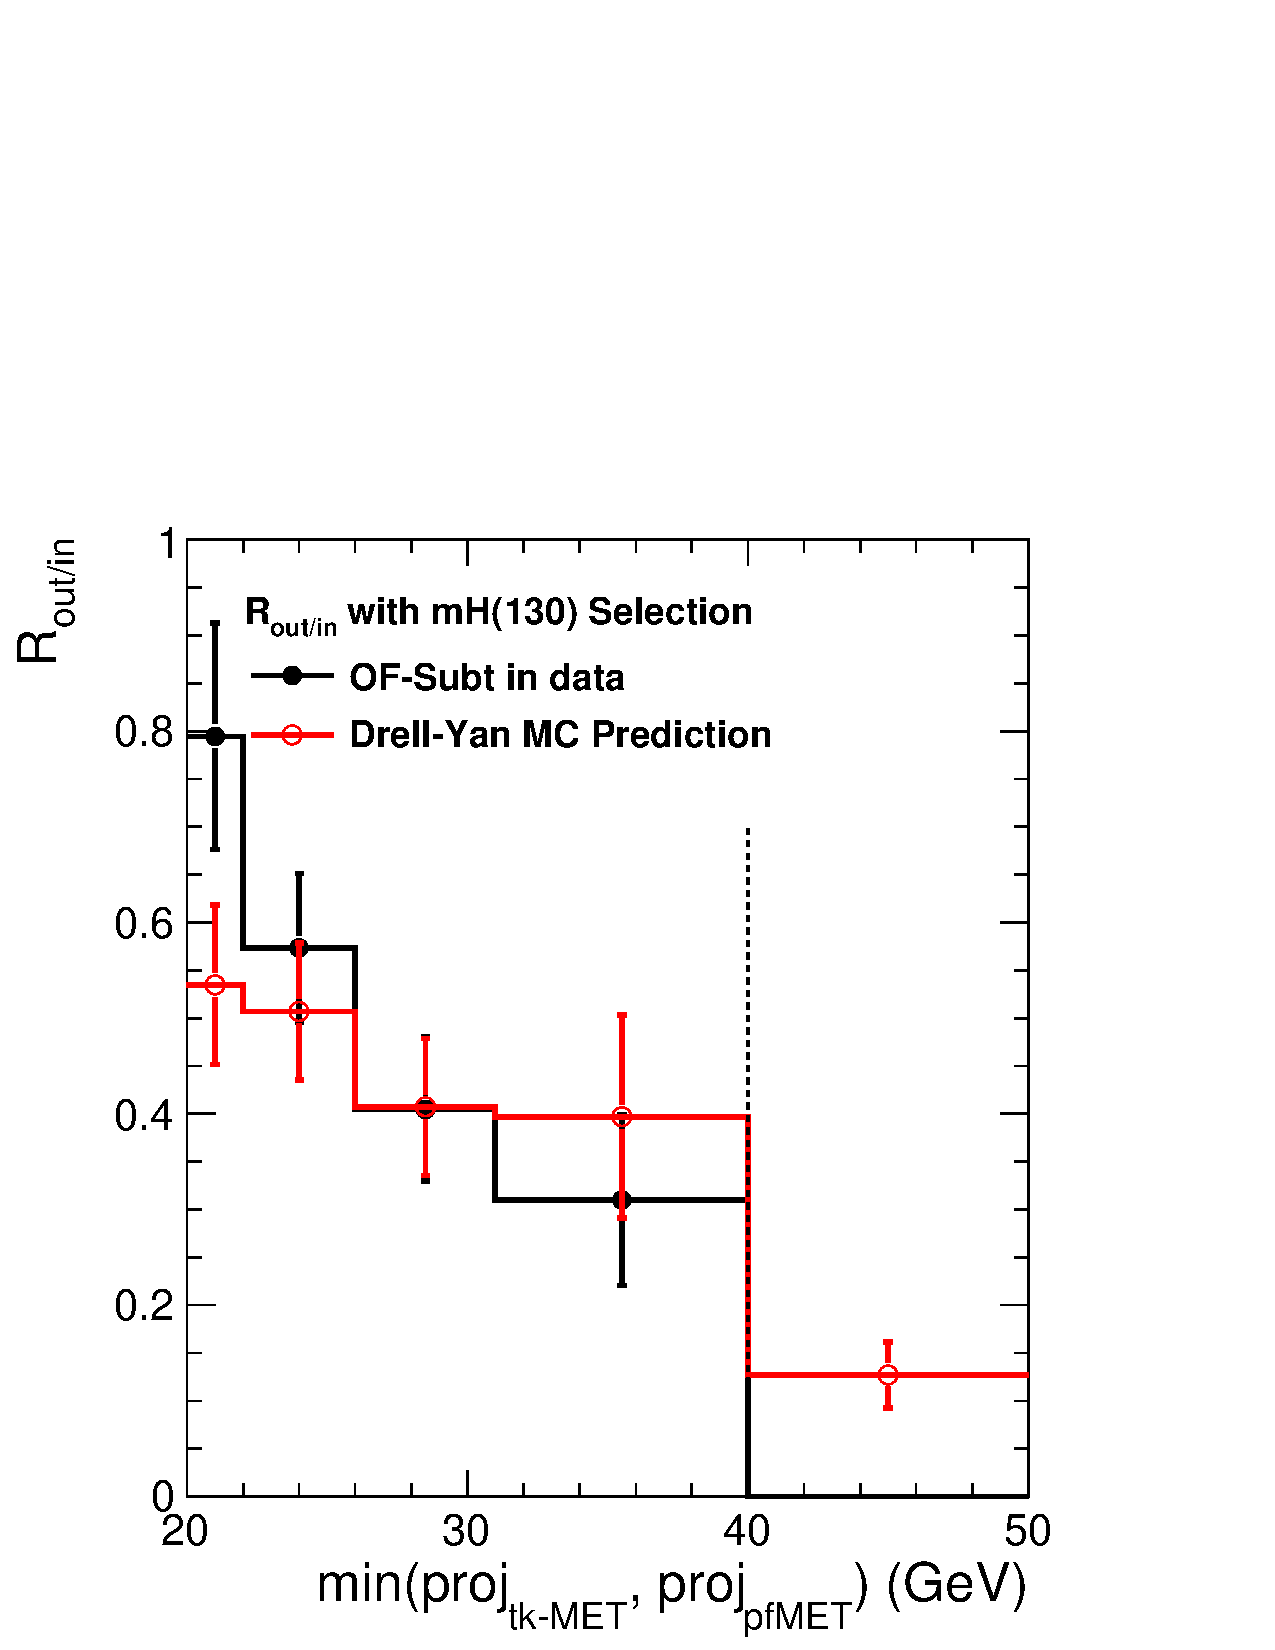
\includegraphics[width=.25\textwidth]{figures/Routin_1Jet_mH130_1092pb_dy.pdf}&
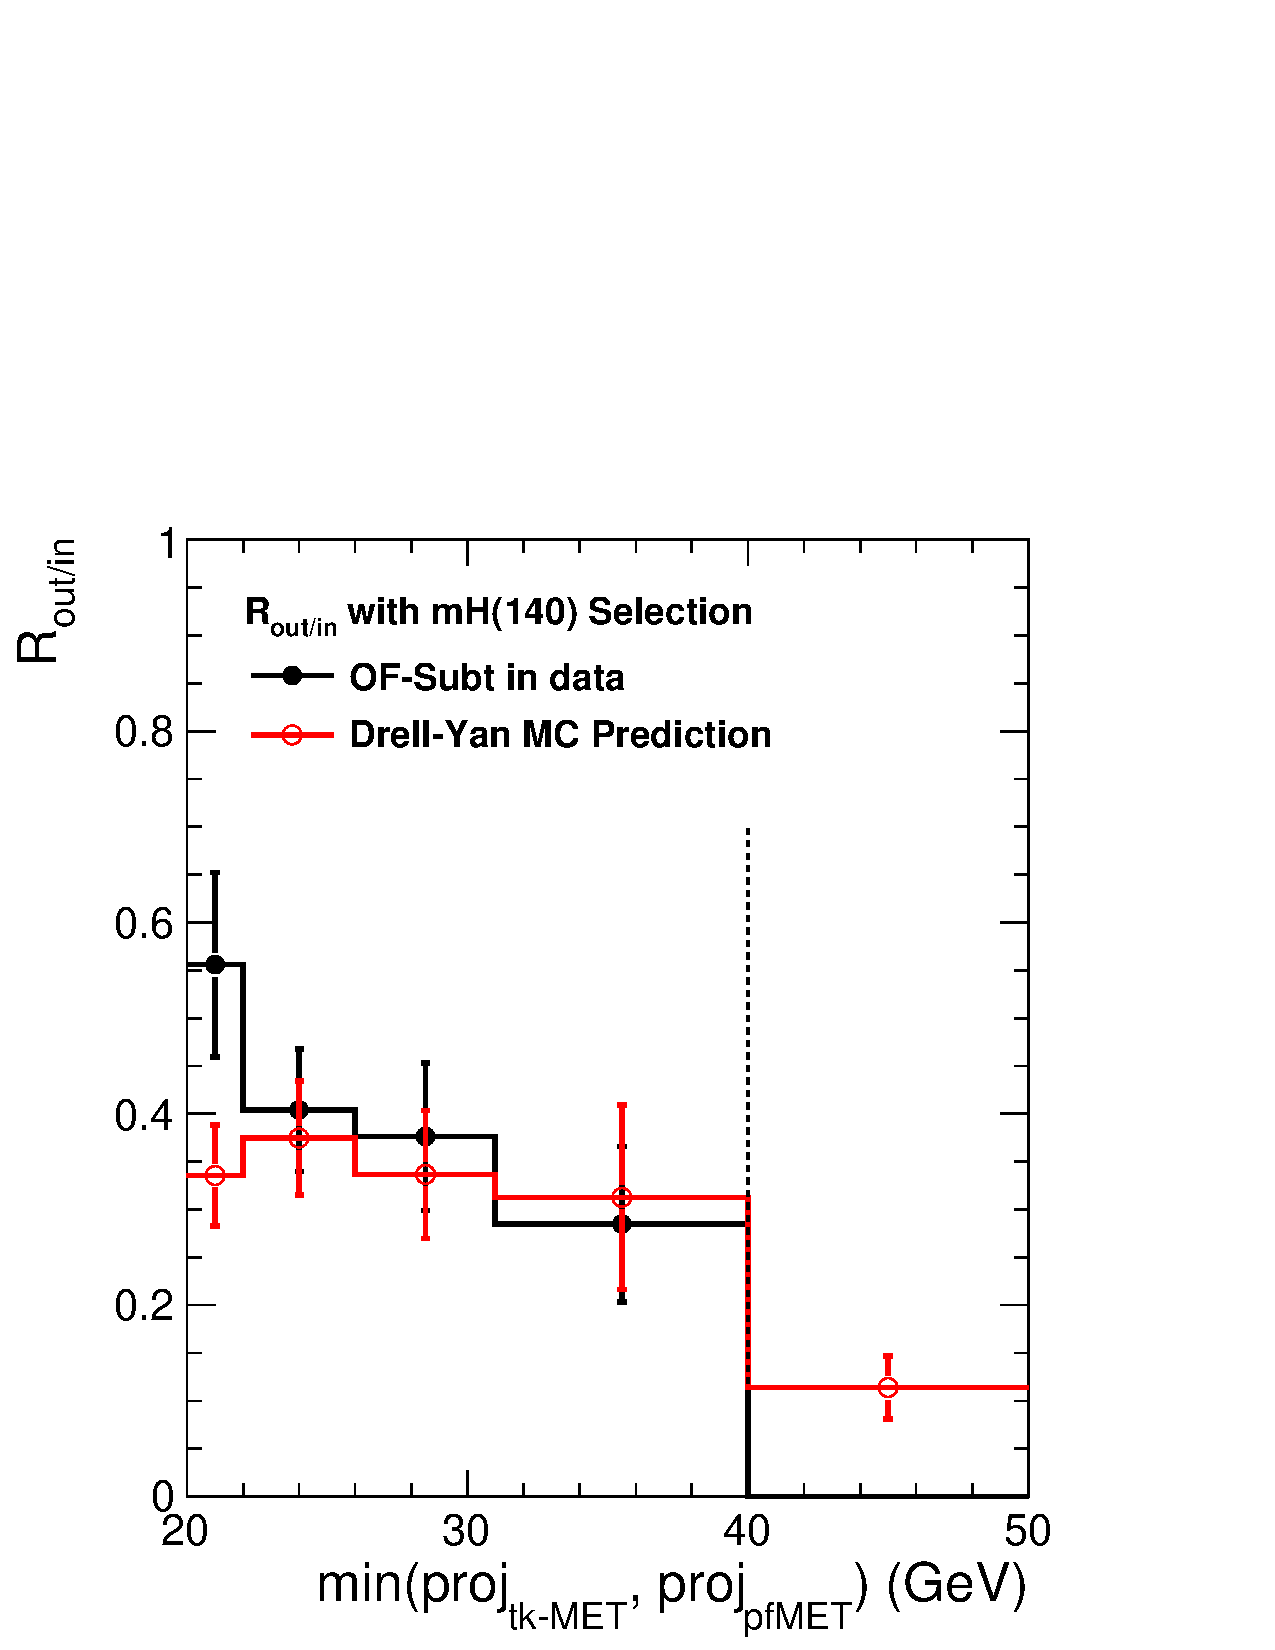
\includegraphics[width=.25\textwidth]{figures/Routin_1Jet_mH140_1092pb_dy.pdf} \\
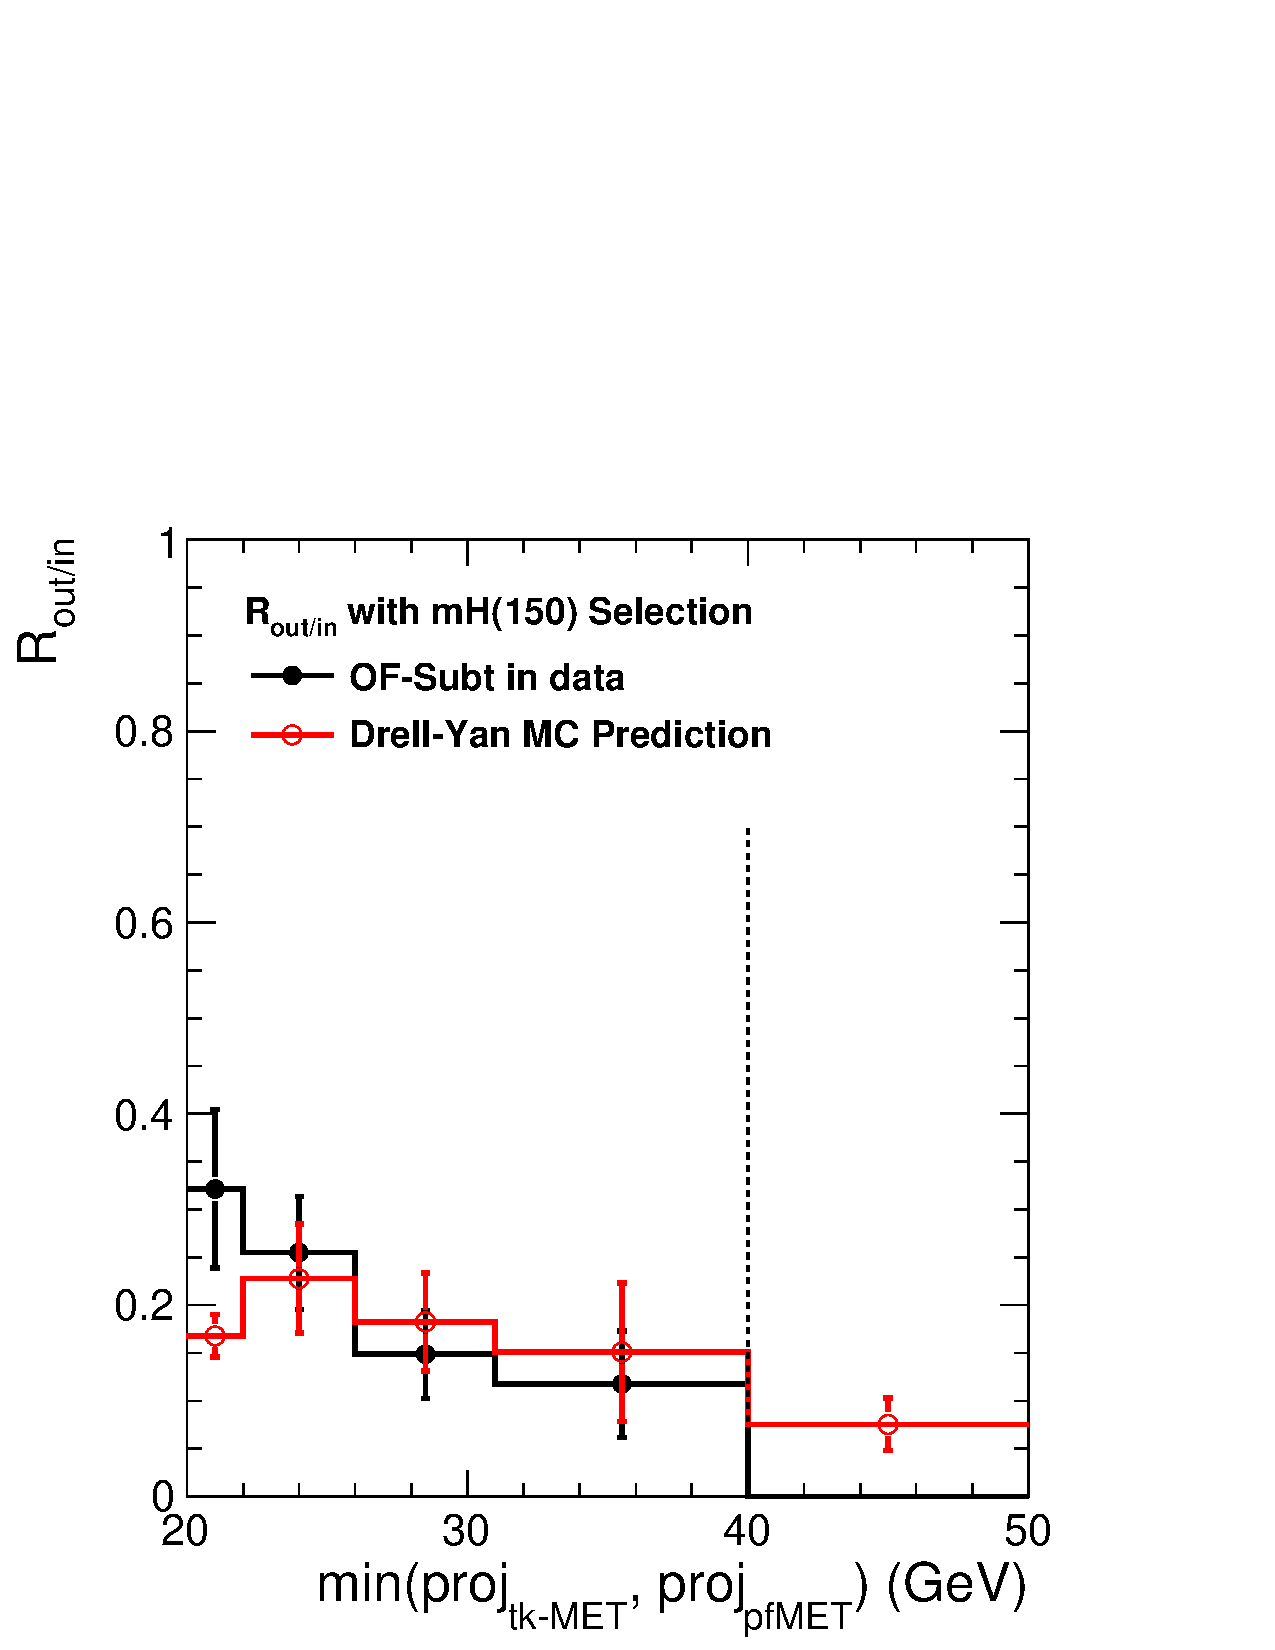
\includegraphics[width=.25\textwidth]{figures/Routin_1Jet_mH150_1092pb_dy.pdf}&
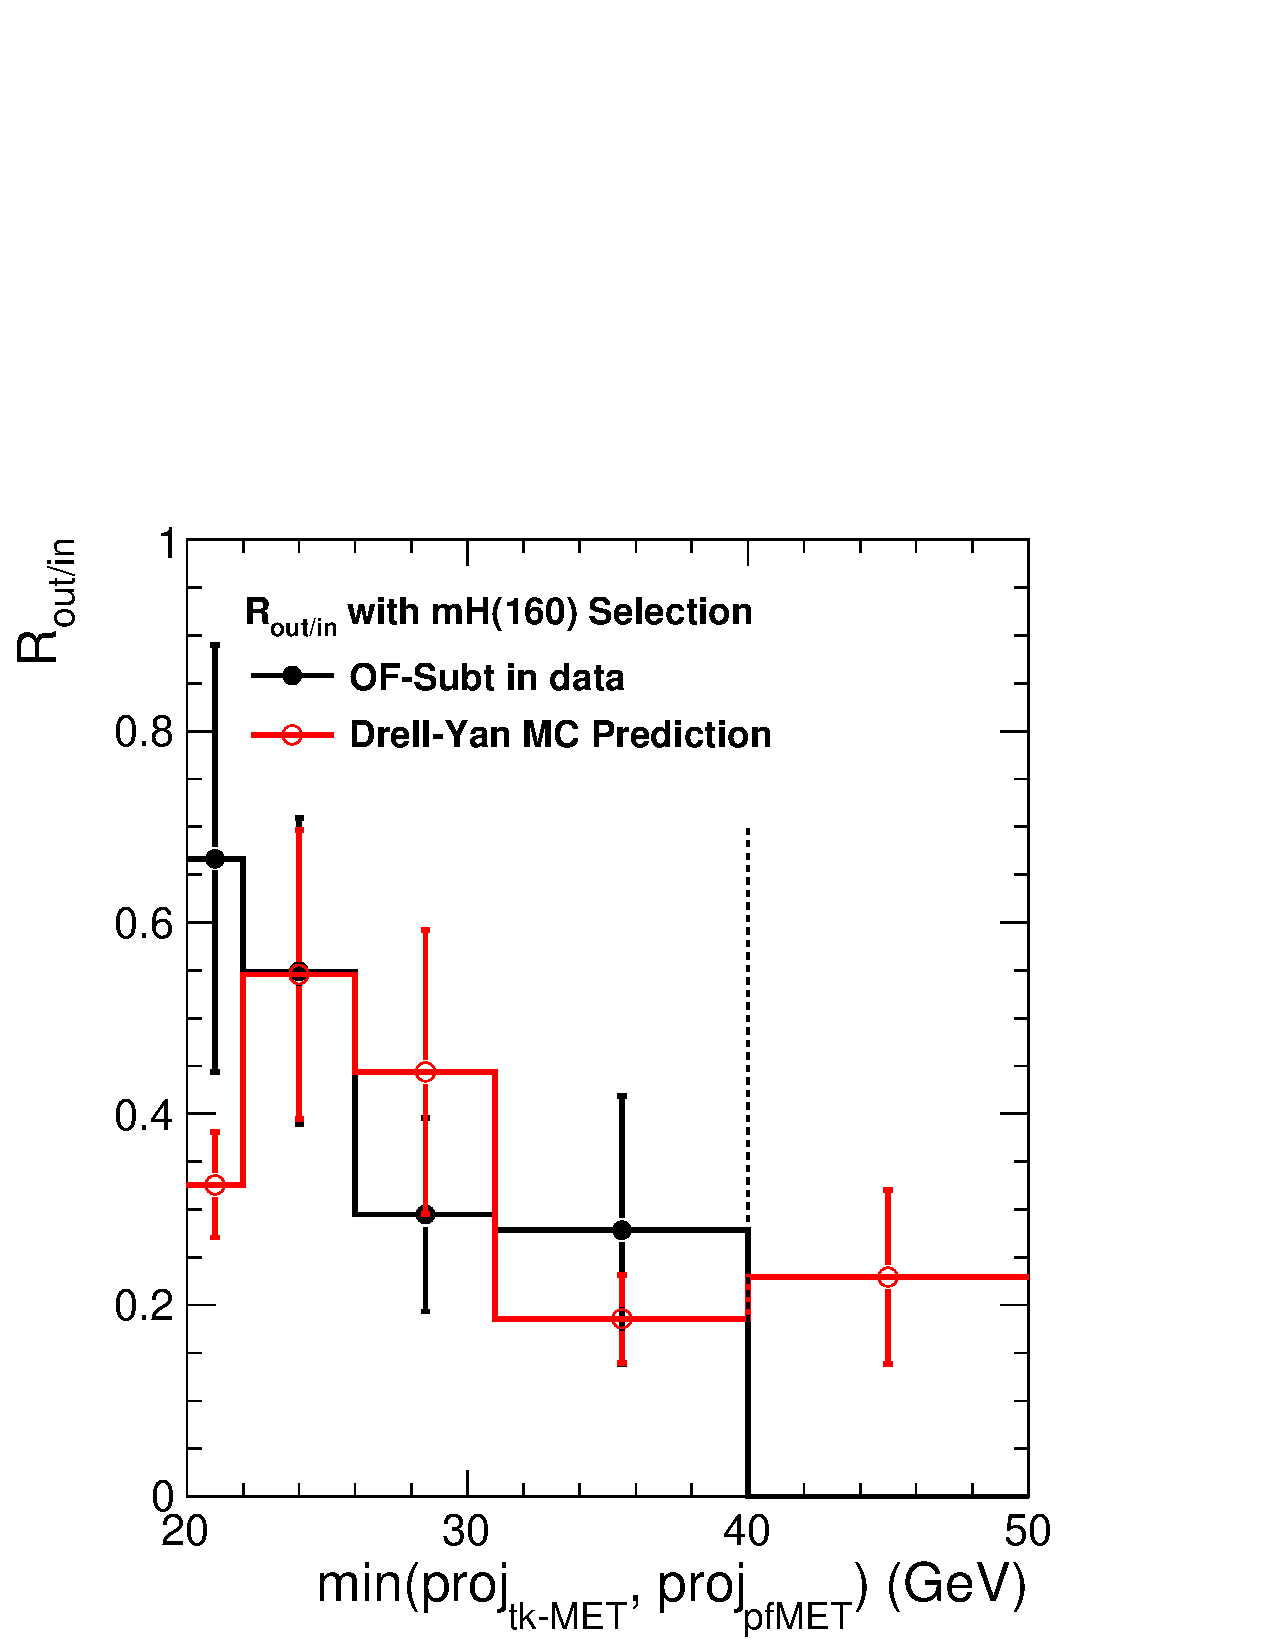
\includegraphics[width=.25\textwidth]{figures/Routin_1Jet_mH160_1092pb_dy.pdf}&
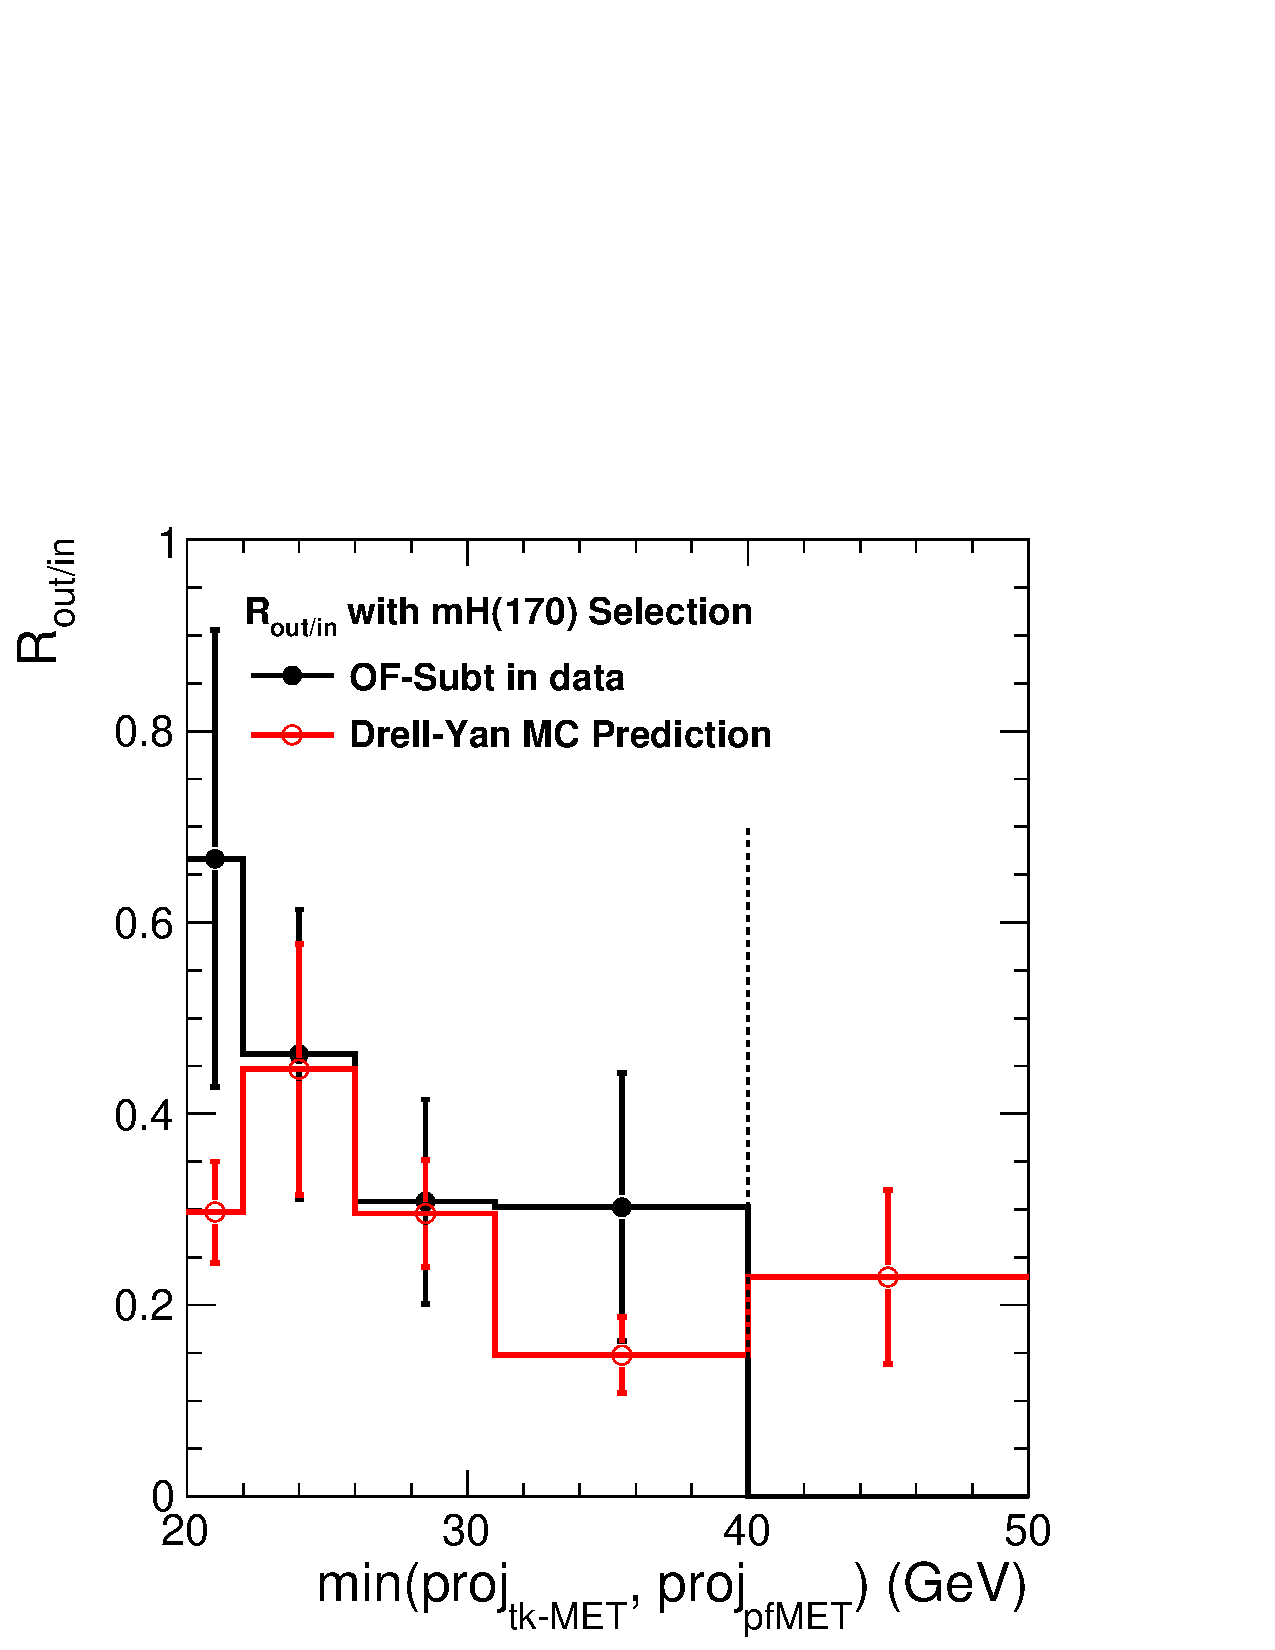
\includegraphics[width=.25\textwidth]{figures/Routin_1Jet_mH170_1092pb_dy.pdf}&
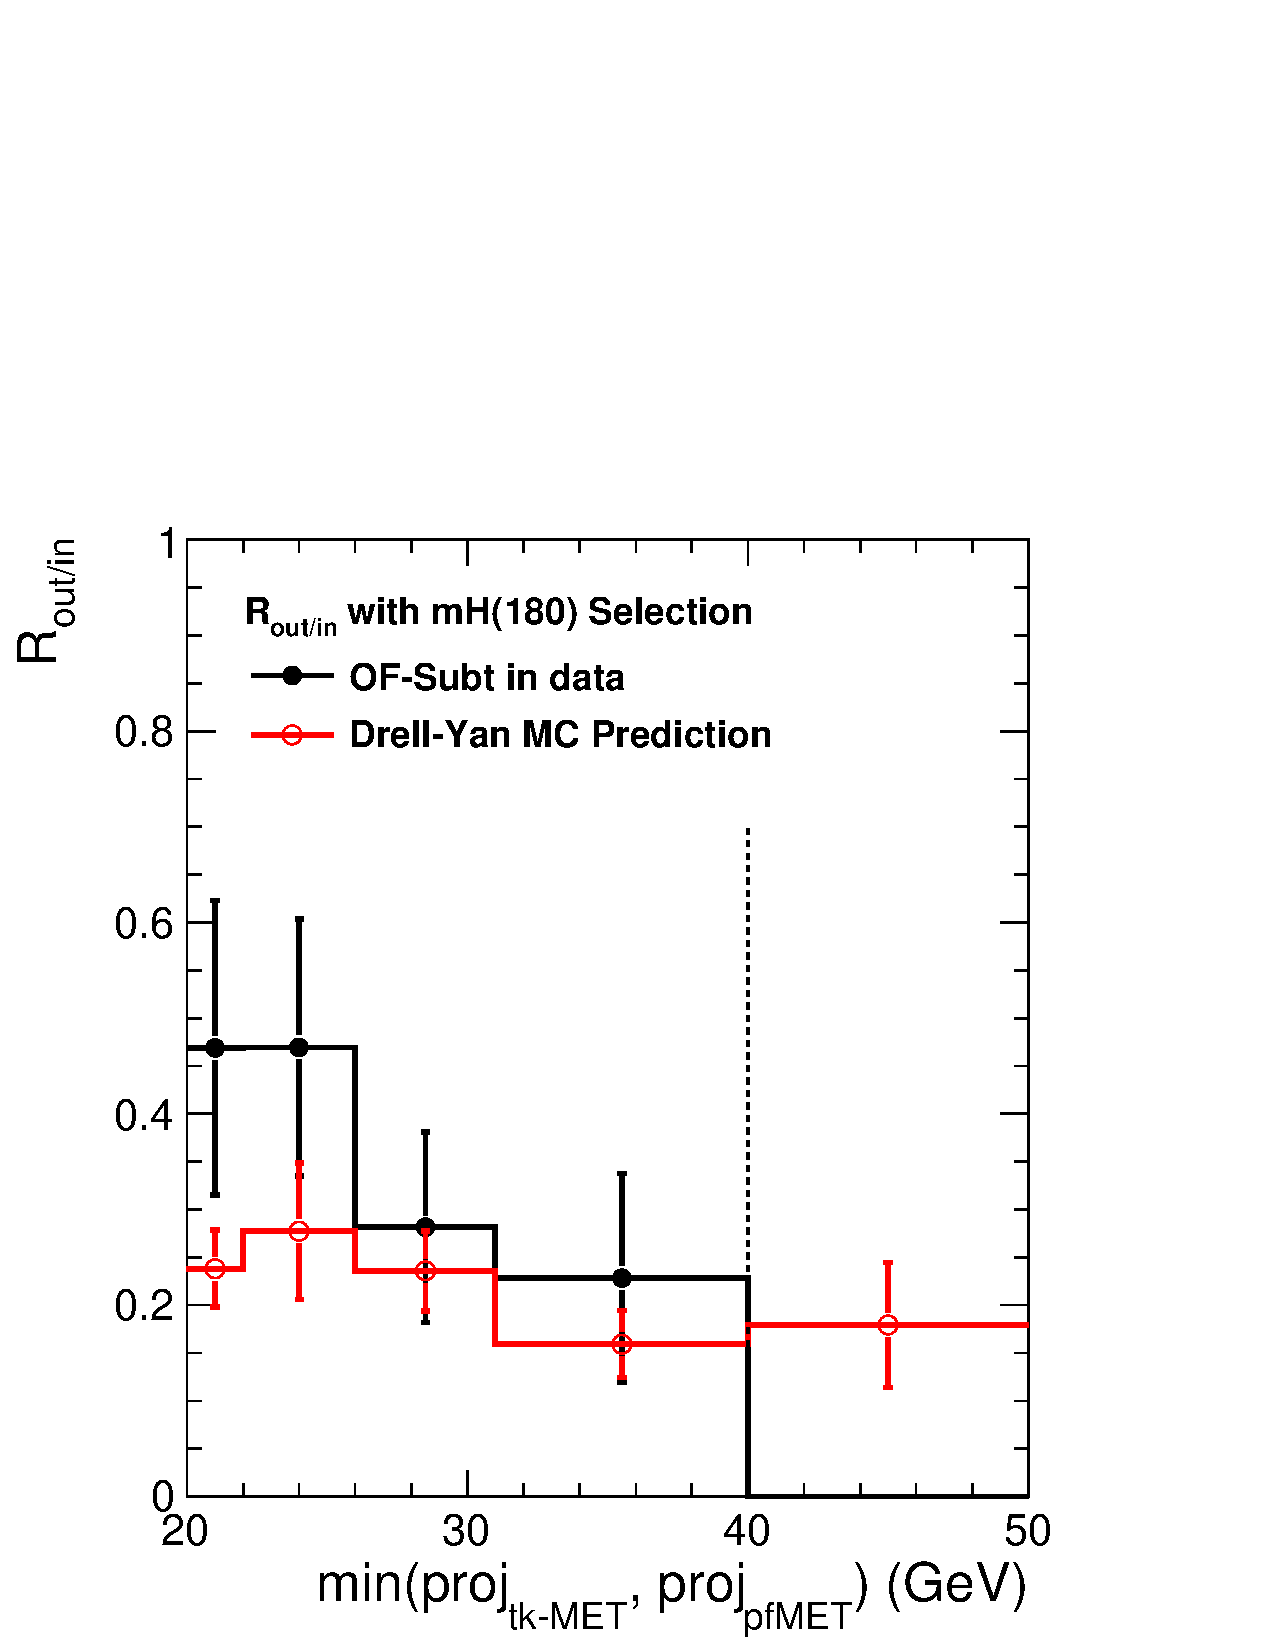
\includegraphics[width=.25\textwidth]{figures/Routin_1Jet_mH180_1092pb_dy.pdf} \\
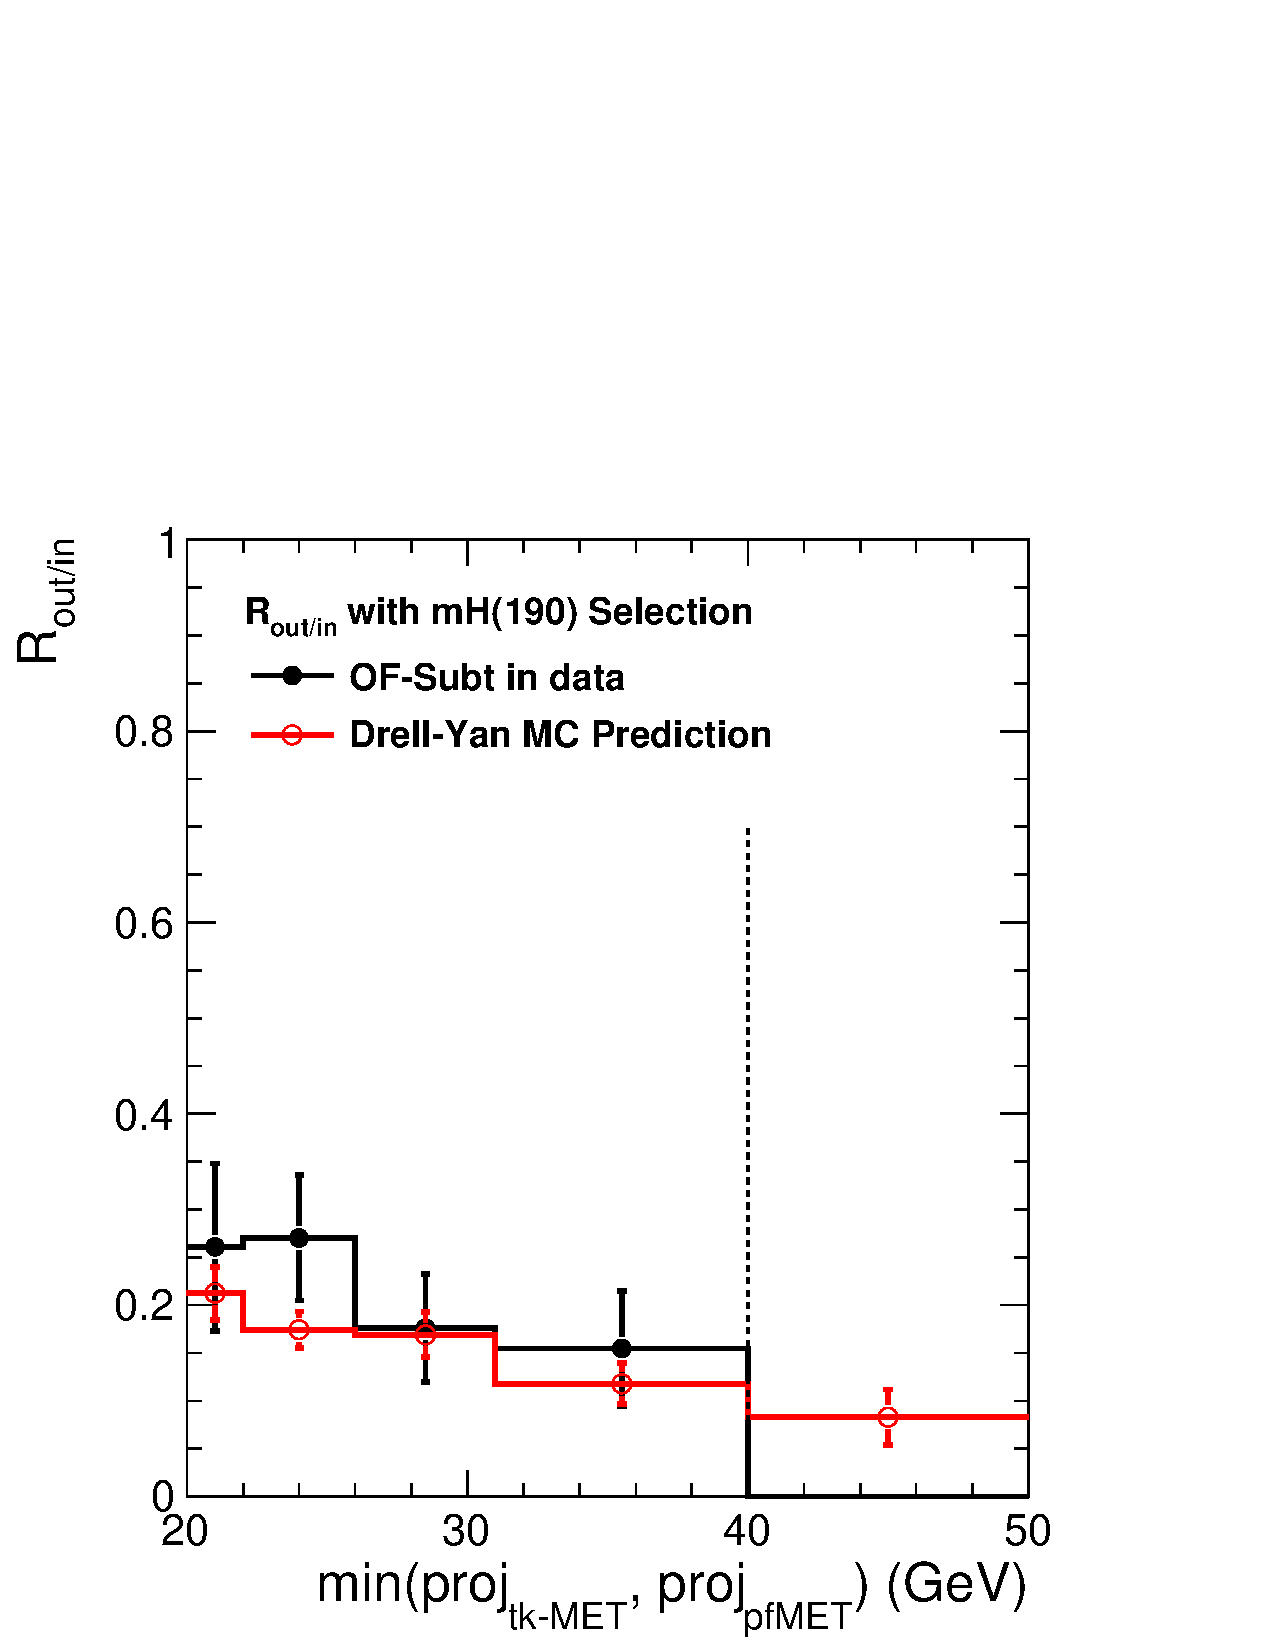
\includegraphics[width=.25\textwidth]{figures/Routin_1Jet_mH190_1092pb_dy.pdf}&
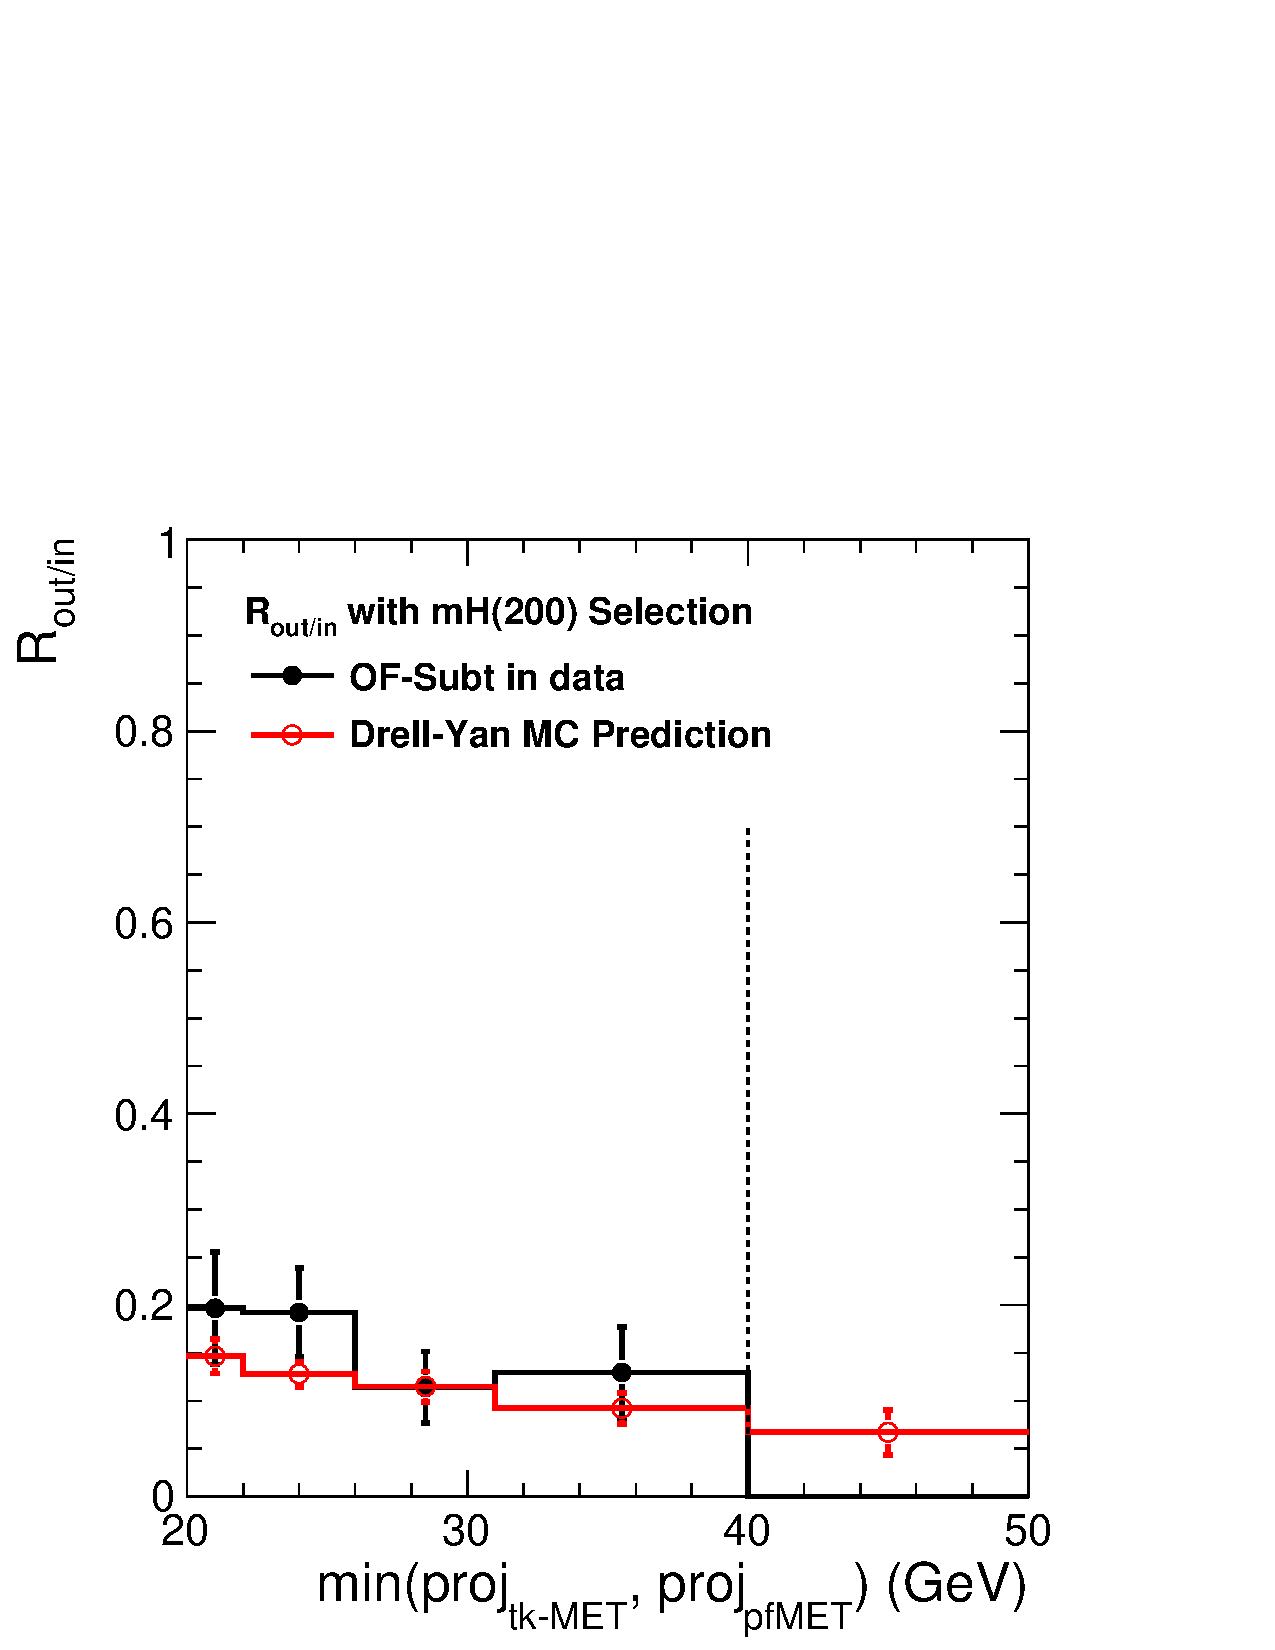
\includegraphics[width=.25\textwidth]{figures/Routin_1Jet_mH200_1092pb_dy.pdf}&
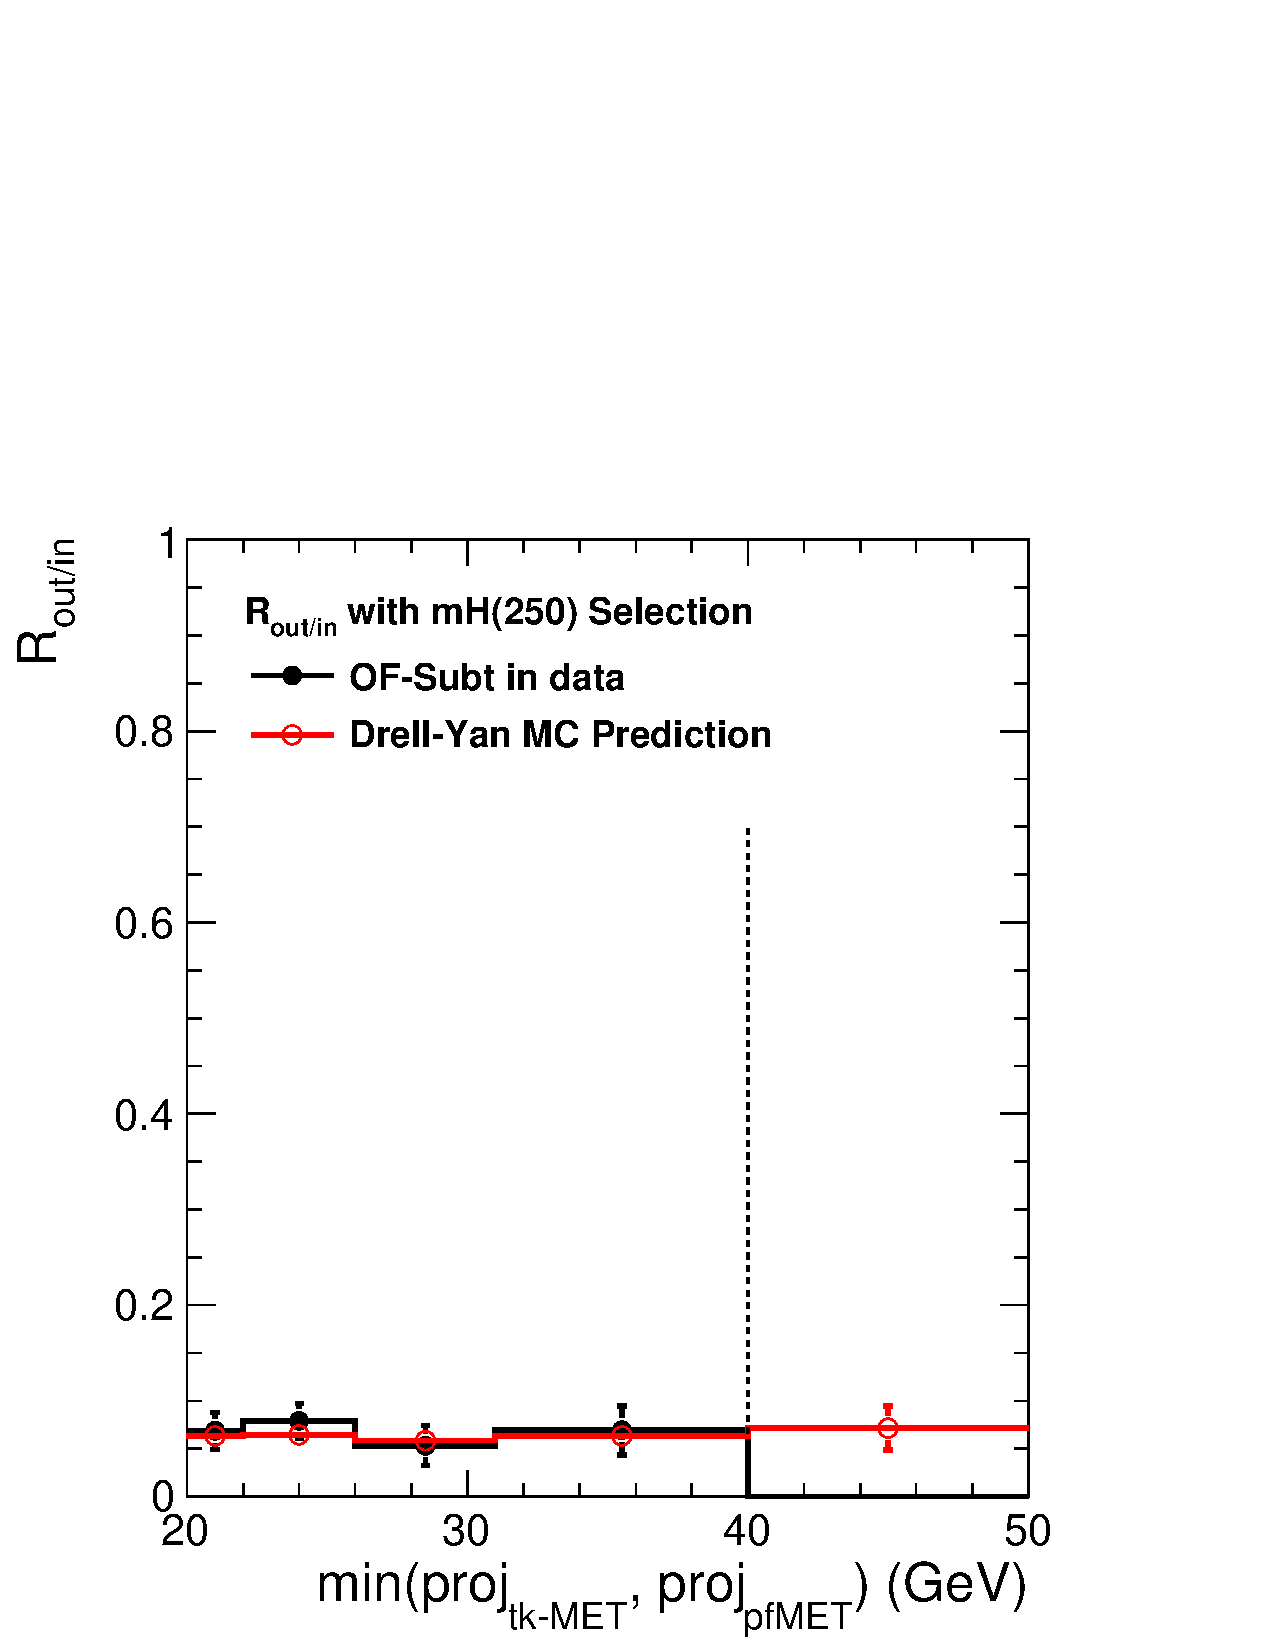
\includegraphics[width=.25\textwidth]{figures/Routin_1Jet_mH250_1092pb_dy.pdf}&
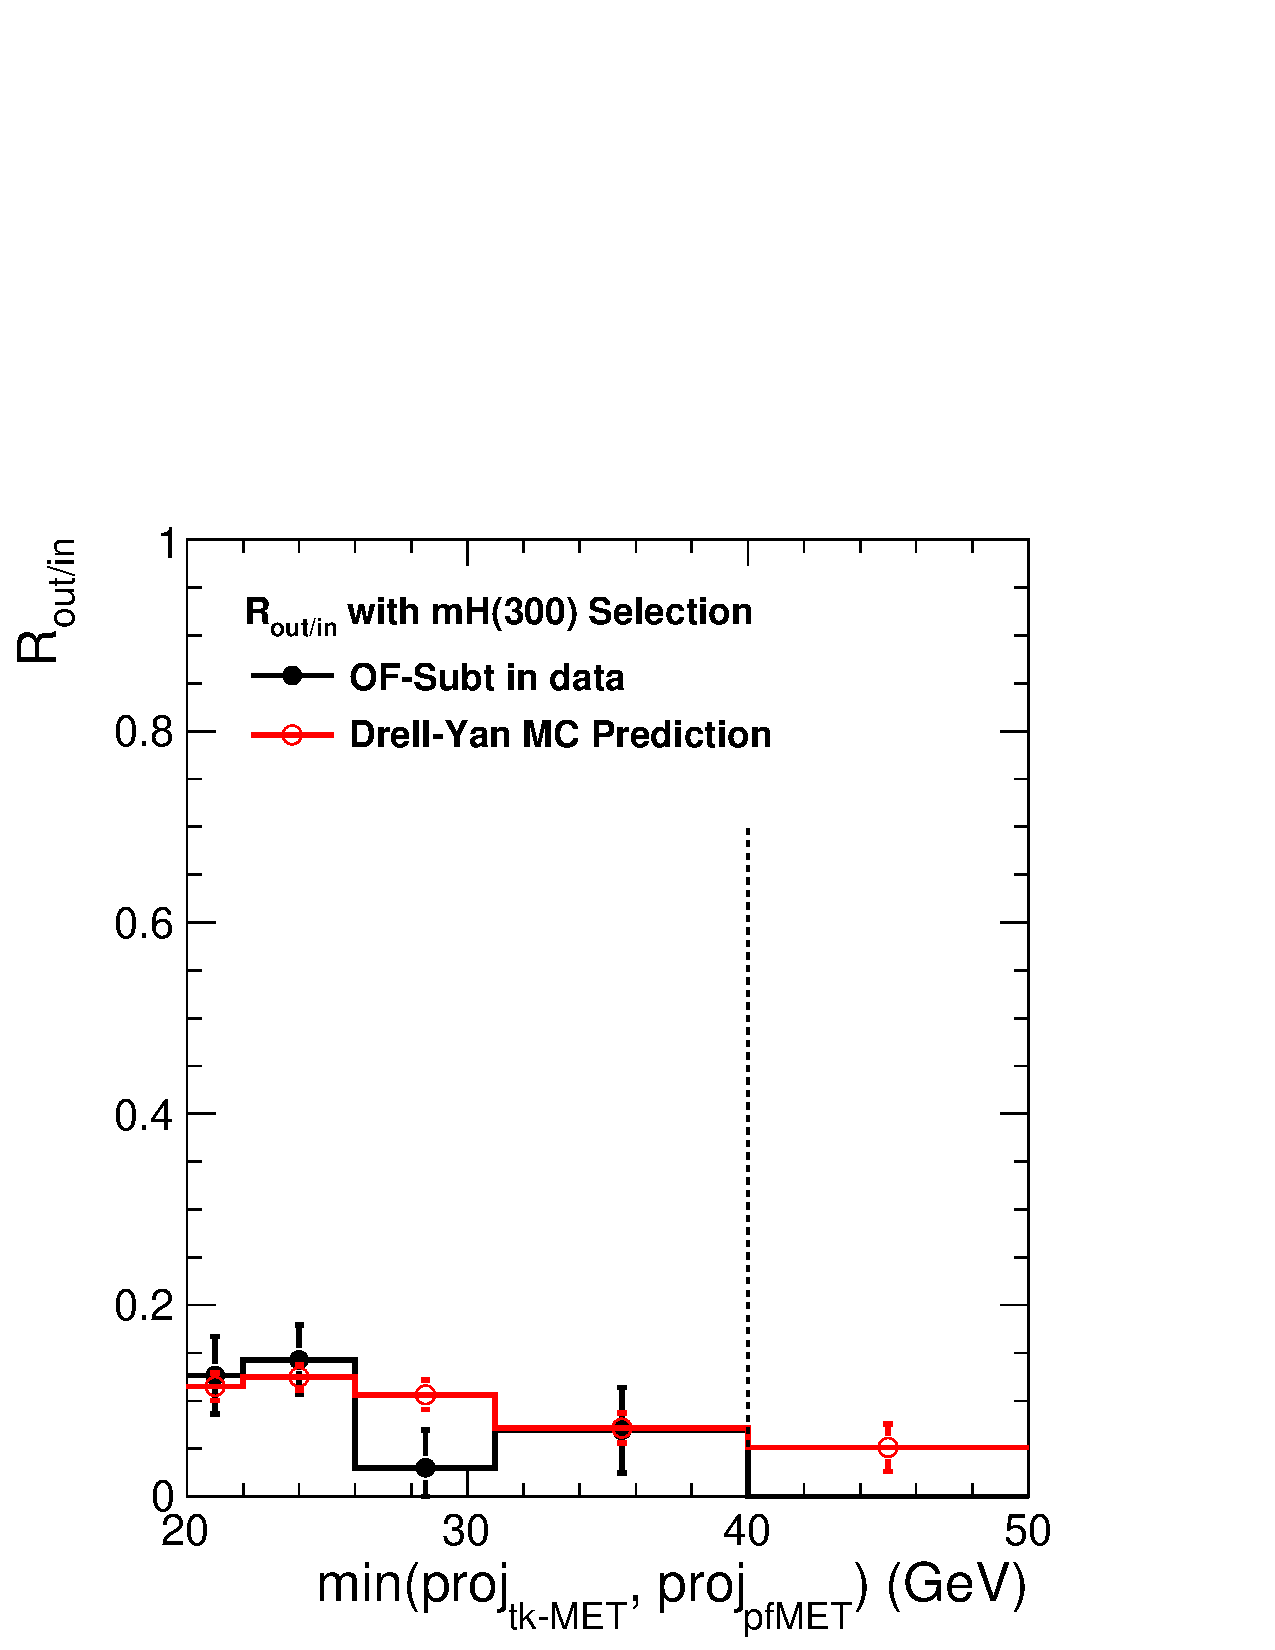
\includegraphics[width=.25\textwidth]{figures/Routin_1Jet_mH300_1092pb_dy.pdf} \\
\end{array}$
\caption{ The \routin\, as a function of MET measured from data (black solid dots)
and MC (red open circles) for the Drell-Yan processes in the 1-Jet bin.
The measurements in data are performed in the control region where we select events
with MET less than the 40 GeV (black dashed line) using the opposite flavor subtraction method.
The MC measurements extend into the signal region shown in the last bin.
The difference in the \routin measurements in different higg selections are due to the
different kinematic cuts applied.
}
\label{fig:routin_1jet}
\end{center}
\end{figure}

